Table~\ref{tab:uncertainties} shows all sources of systematic uncertainty currently considered in the analysis.
\begin{table}[h!]
  \centering
  \begin{tabular}{lll}\hline
Source                          & Channel     & Size \\\hline
\multicolumn{3}{l}{\bf Experimental uncertainties} \\
Luminosity                      & all         & 1.026 \\
Loose lepton efficiency         &             & 1.02 per lepton  \\
Tight lepton efficiency         &             & 1.03 per lepton  \\
Trigger efficiency              & \mumu\      & 1.01 \\
                                & \emu\       & 1.01 \\
                                & \ee\        & 1.02 \\
                                & \threel\    & 1.03 \\
Jet energy scale                & all         & templates \\
Forward jet modeling            & all         & templates, see Tab.~\ref{tab:ratioFwdJet} \\
\cPqb\ tagging efficiency       & all         & templates \\ \hline

\multicolumn{3}{l}{\bf Theory uncertainties} \\
$Q^2$ scale (\tHq)              & all         & 0.92--1.06 (depending on \Ct, \CV)\\
$Q^2$ scale (\tHW)              & all         & 0.93--1.05 (depending on \Ct, \CV)\\
$Q^2$ scale (\ttH)              & all         & 0.915/1.058\\
$Q^2$ scale (\ttW)              & all         & 1.12\\
$Q^2$ scale (\ttZ)              & all         & 1.11\\
pdf (\ttH)                      & all         & 1.036\\
pdf $\Pg\Pg$ (\ttZ)             & all         & 0.966\\
pdf $\Pq\Paq$ (\ttW)            & all         & 1.04\\
pdf $\Pq\Pg$ (\tHq)             & all         & 1.037\\
pdf $\Pq\Pg$ (\tHW)             & all         & 1.040\\ \hline
\multicolumn{3}{l}{\bf Higgs branching fractions} \\
\verb|param_alphaS|             & all         & 1.012\\
\verb|param_mB|                 & all         & 0.981\\
\verb|HiggsDecayWidthTHU_hqq|   & all         & 0.988\\
\verb|HiggsDecayWidthTHU_hvv|   & all         & 1.004\\
\verb|HiggsDecayWidthTHU_hll|   & all         & 1.019\\\hline

\multicolumn{3}{l}{\bf Backgrounds}         \\
\WZ\ control region statistics  & \threel\    & 1.10 \\
\WZ\ control region backgrounds & \threel\    & 1.20 \\
\WZ\ modeling                   & \threel\    & 1.07  \\
$\WZ+2\text{jet}$ background    & \mumu,\emu\ & 1.50 \\
Rare SM processes               & all         & 1.50 \\
Charge flips                    & \emu\       & 1.30 \\\hline
\multicolumn{3}{l}{\bf Fake rate estimate}     \\
Electron FR measurement         &             & templates \\
Muon FR measurement             &             & templates \\
Electron closure                & \ee\        & 1.05 norm., (0.99 (\ttbar)/1.06 (\ttV)) shape var. \\
                                & \emu\       & 0.94 norm., (0.98 (\ttbar)/1.07 (\ttV)) shape var. \\
                                & \threel\    & 1.40 norm., (1.09 (\ttbar)/1.05 (\ttV)) shape var. \\
Muon closure                    & \mumu\      & 1.07 norm., (0.97 (\ttbar)/0.91 (\ttV)) shape var. \\
                                & \emu\       & 1.09 norm., (1.06 (\ttbar)/1.03 (\ttV)) shape var. \\
                                & \threel\    & 1.09 norm., (0.95 (\ttbar)/0.83 (\ttV)) shape var. \\\hline
   \end{tabular} 
   \caption{Pre-fit size of systematic uncertainties.}\label{tab:uncertainties}
 \end{table}

\textbf{Experimental uncertainties}
A normalization uncertainty is derived from the measurement of data/MC scale factors for lepton and trigger efficiencies.
Jet energy scale uncertainties and \cPqb\ tagging efficiency are evaluated using dedicated shape templates derived from a variation of the jet energy scale within its uncertainty and from varying the \cPqb\ tagging data/MC scale factors within their uncertainty.

The forward jet $\eta$ distribution is poorly modeled in simulation, see Appendix~\ref{app:fwdcontrol}.
To estimate the effect of a mismodeled forward jet distribution, we reweight the events in simulation (\ie\ for signal and the irreducible backgrounds) based on the normalized data/MC ratio in the control region and thereby derive an alternative shape of the BDT output distributions that reflects a hypothetical perfect data/MC agreement.

\textbf{Theory uncertainties}
$Q^2$ scale and parton distribution function (pdf) uncertainties are applied as an overall normalization uncertainty using numbers from the NLO theory calculation.

\textbf{Backgrounds}
In addition to the theory uncertainties on the main irreducible backgrounds of \ttW, \ttZ, and \ttH, the smaller irreducible backgrounds and the charge mis-identification estimate are covered with flat normalization uncertainties.
The \WZ\ contribution is normalized in a data control region and an uncertainty on the scale factor is derived in the process.
Finally, the dominant uncertainty relates to the estimate of the reducible non-prompt lepton contribution using a fake rate method.
The main normalization uncertainty on the used fake rates derives from limited statistics in the data control region, and the subtraction of residual prompt lepton contribution, see Ref.~\cite{CMS_AN_2017-029}.
Furthermore, shape variations resembling data/MC differences and deviations in closure test are evaluated as shape uncertainties.

\textbf{Fake rate closure uncertainties}
The BDT output shapes are compared between a pure MC estimation of fake leptons (in \ttbar), and an application of fake-rates as measured in QCD MC, applied in \ttbar\ MC events.
The difference in the resulting normalization and output shapes, both the training vs. \ttbar\ and vs. \ttV, are estimated and propagated to the fit as normalization and shape variations.
See Figs~\ref{fig:frclosure_2lss_ee} to~\ref{fig:frclosure_3l_mufake} for the results of these closure tests and Tab.~\ref{tab:uncertainties} for the resulting pre-fit uncertainties.

\begin{figure}[htb]
 \centering
 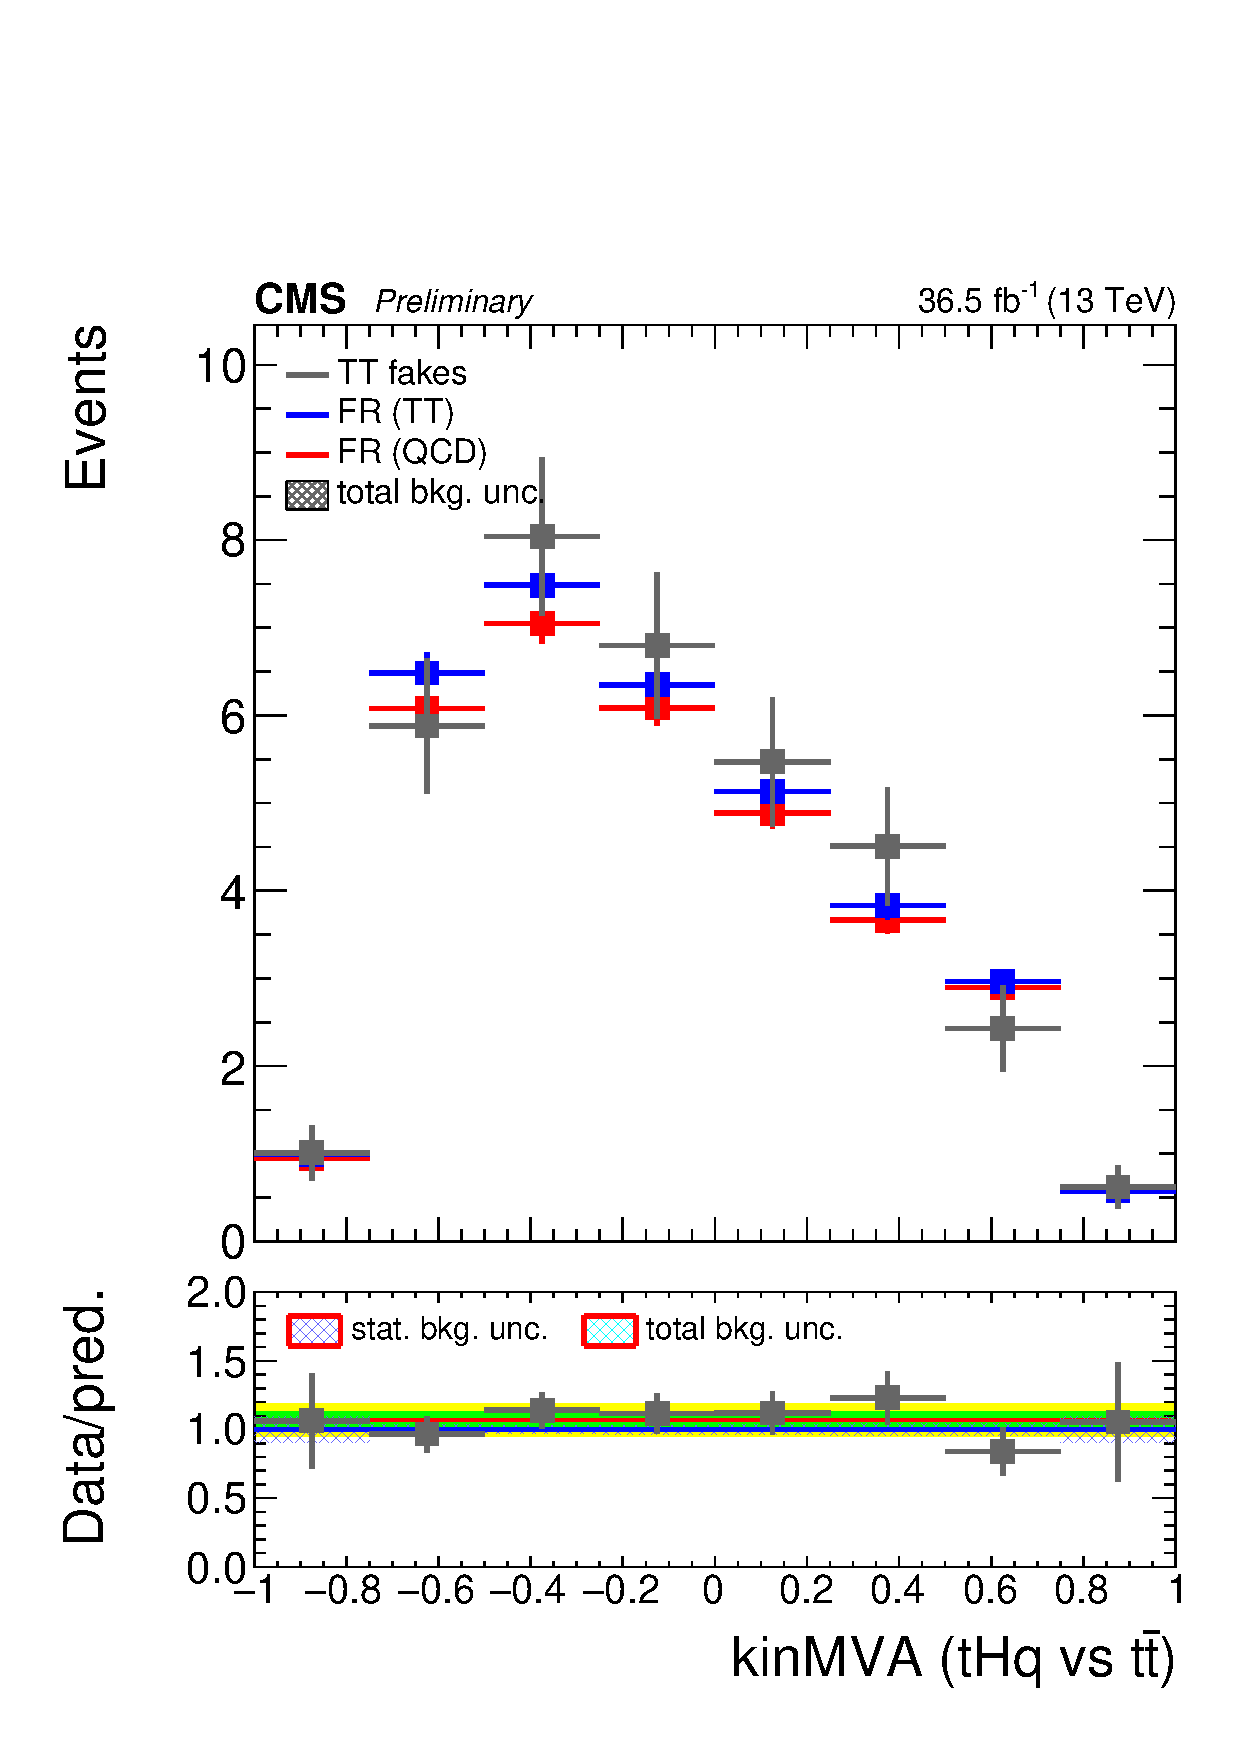
\includegraphics[width=0.245\textwidth]{figures/FR_closures/thqMVA_tt_2lss_ee_norm.pdf} 
 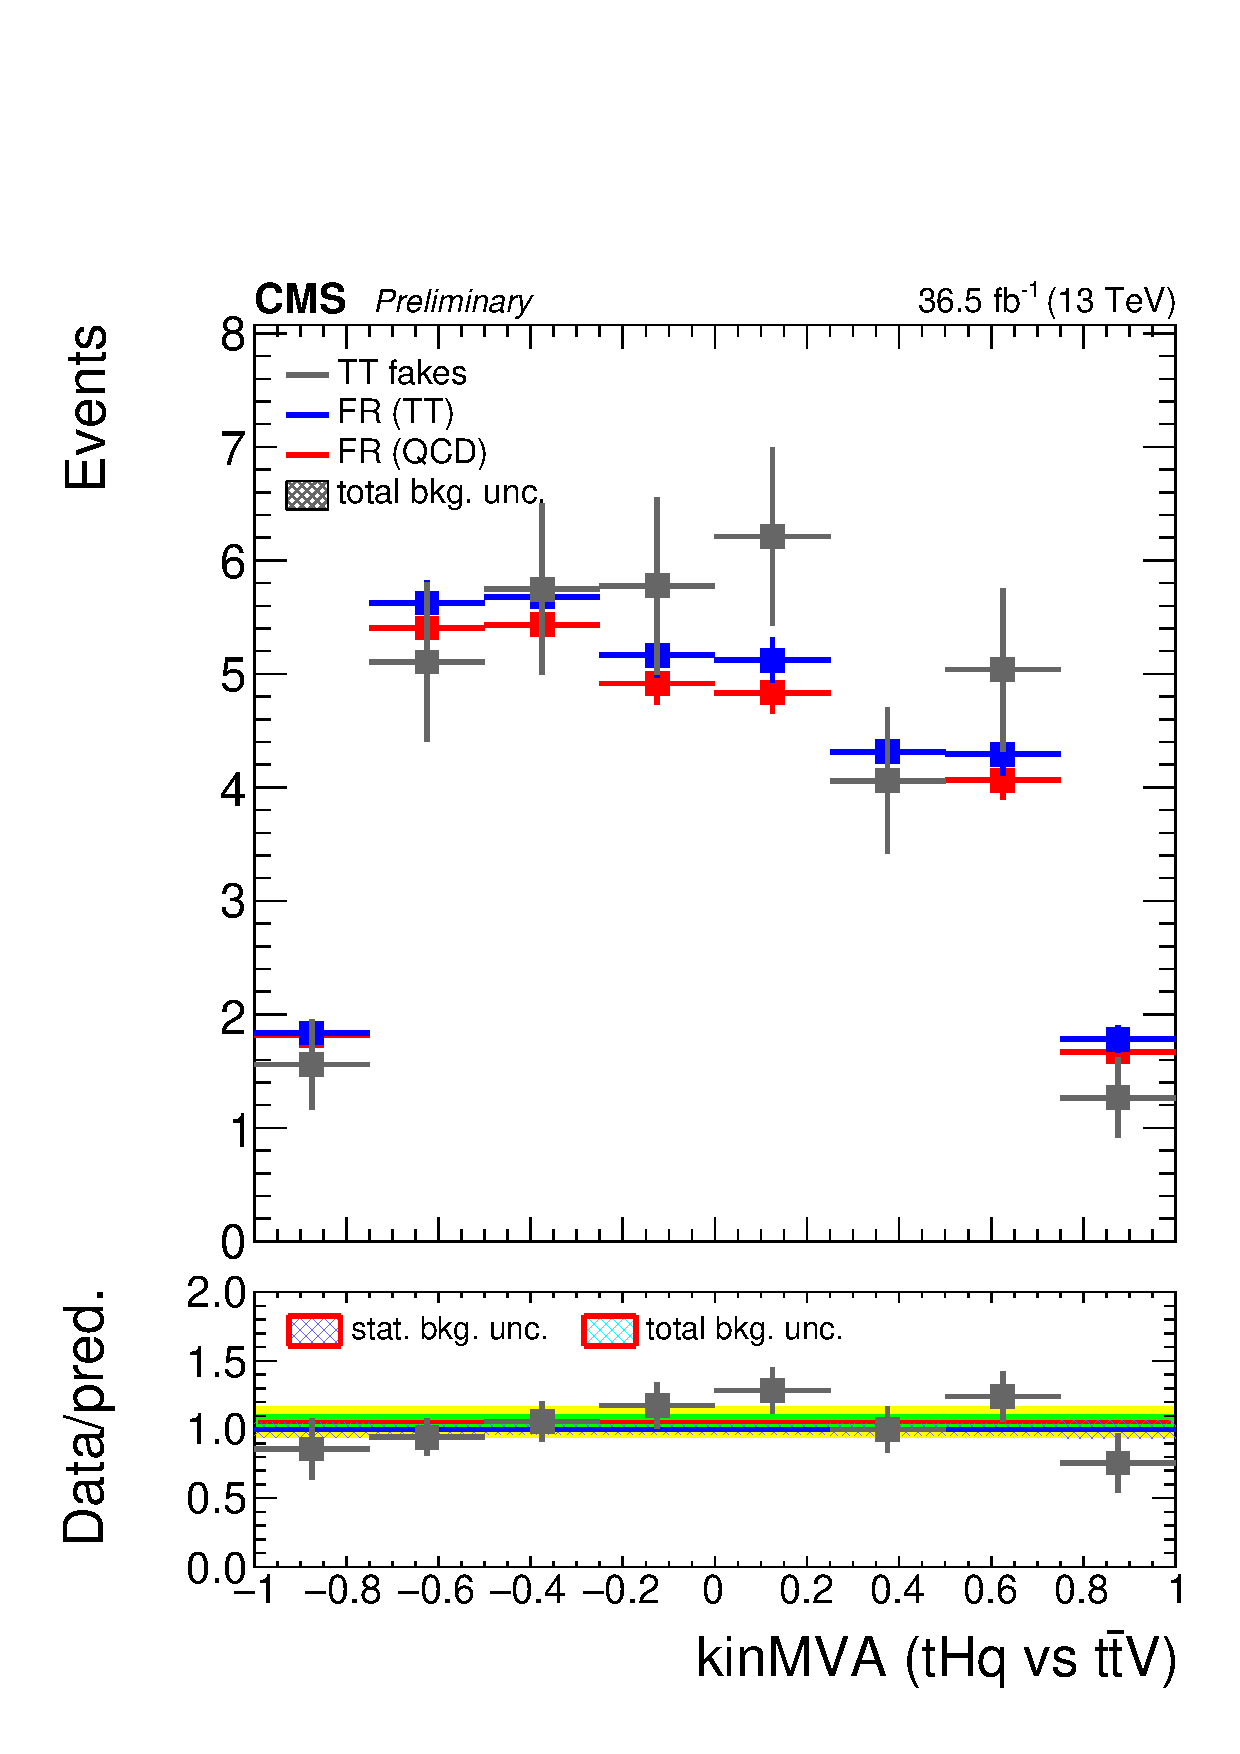
\includegraphics[width=0.245\textwidth]{figures/FR_closures/thqMVA_ttv_2lss_ee_norm.pdf} 
 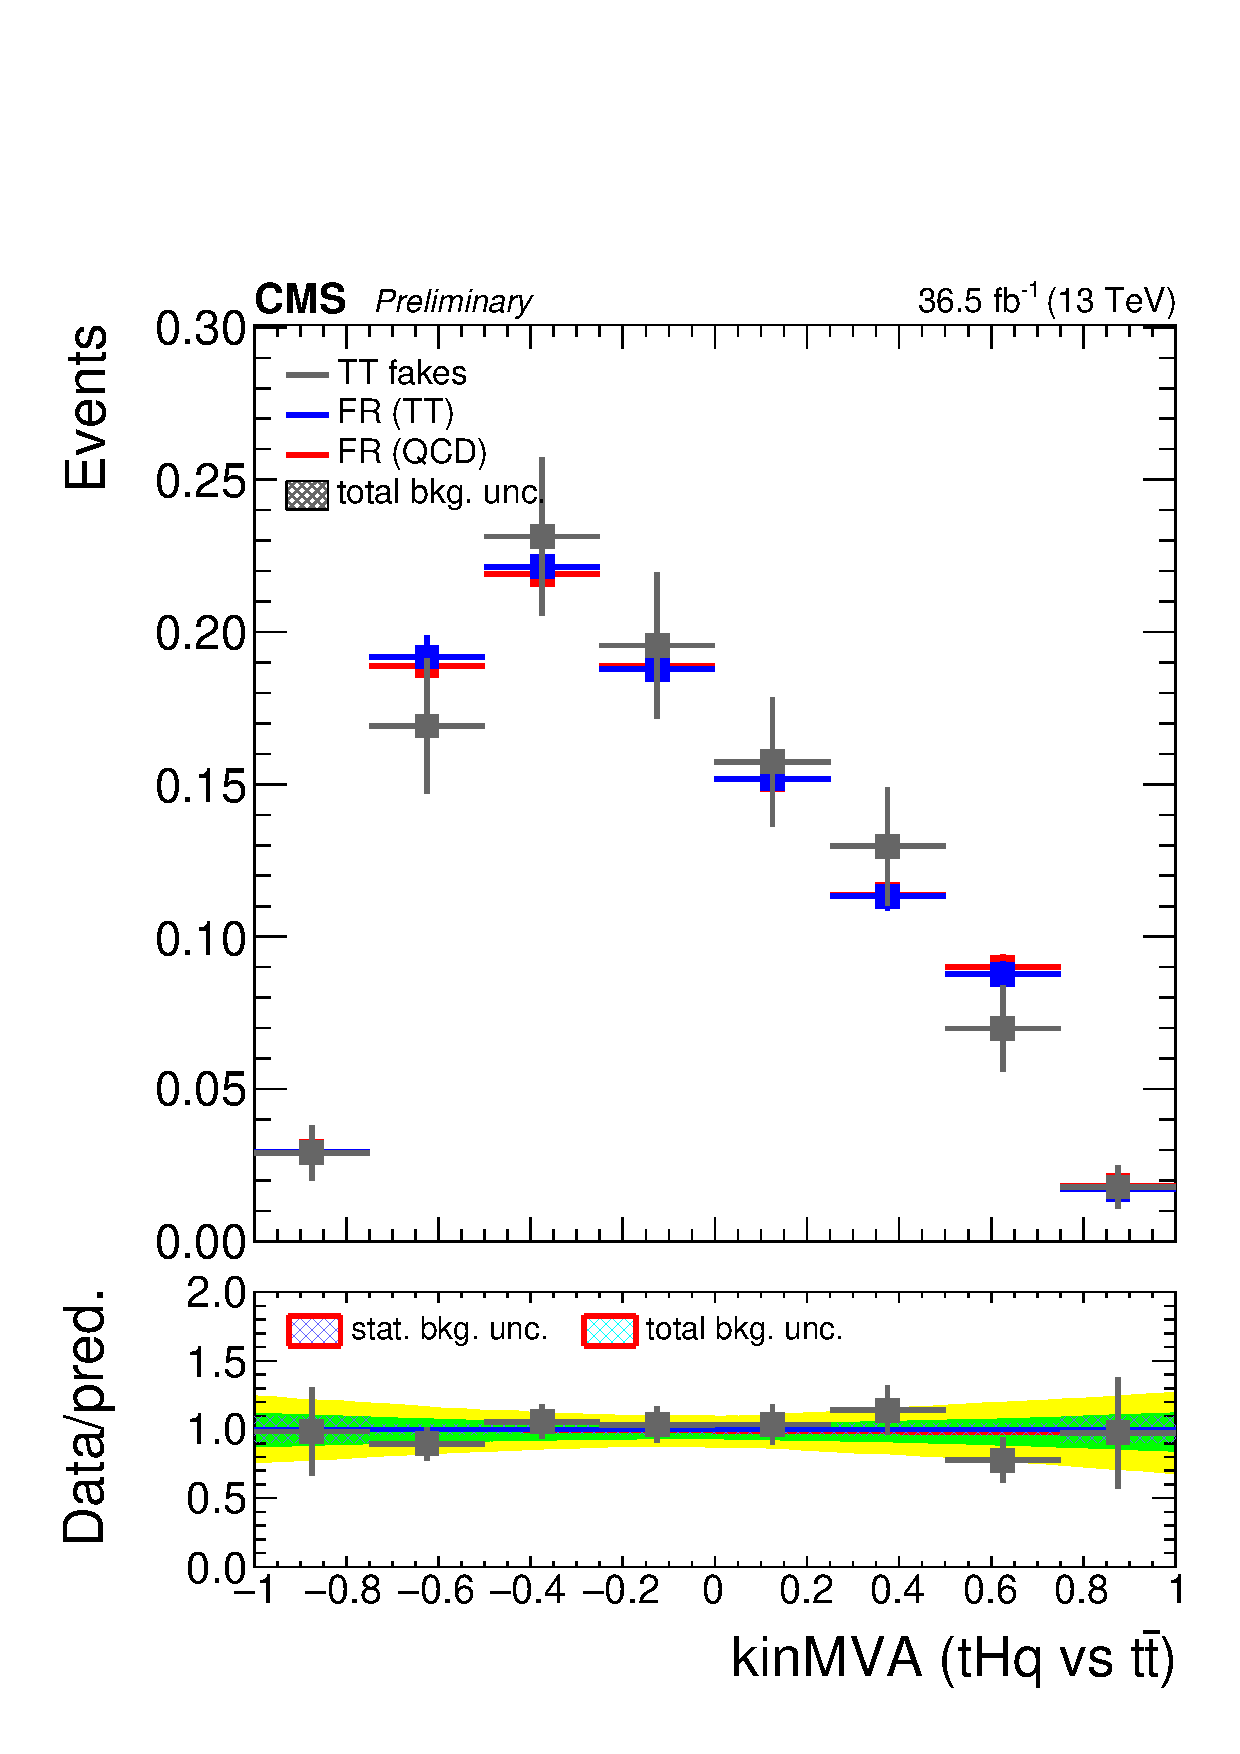
\includegraphics[width=0.245\textwidth]{figures/FR_closures/thqMVA_tt_2lss_ee_shape.pdf} 
 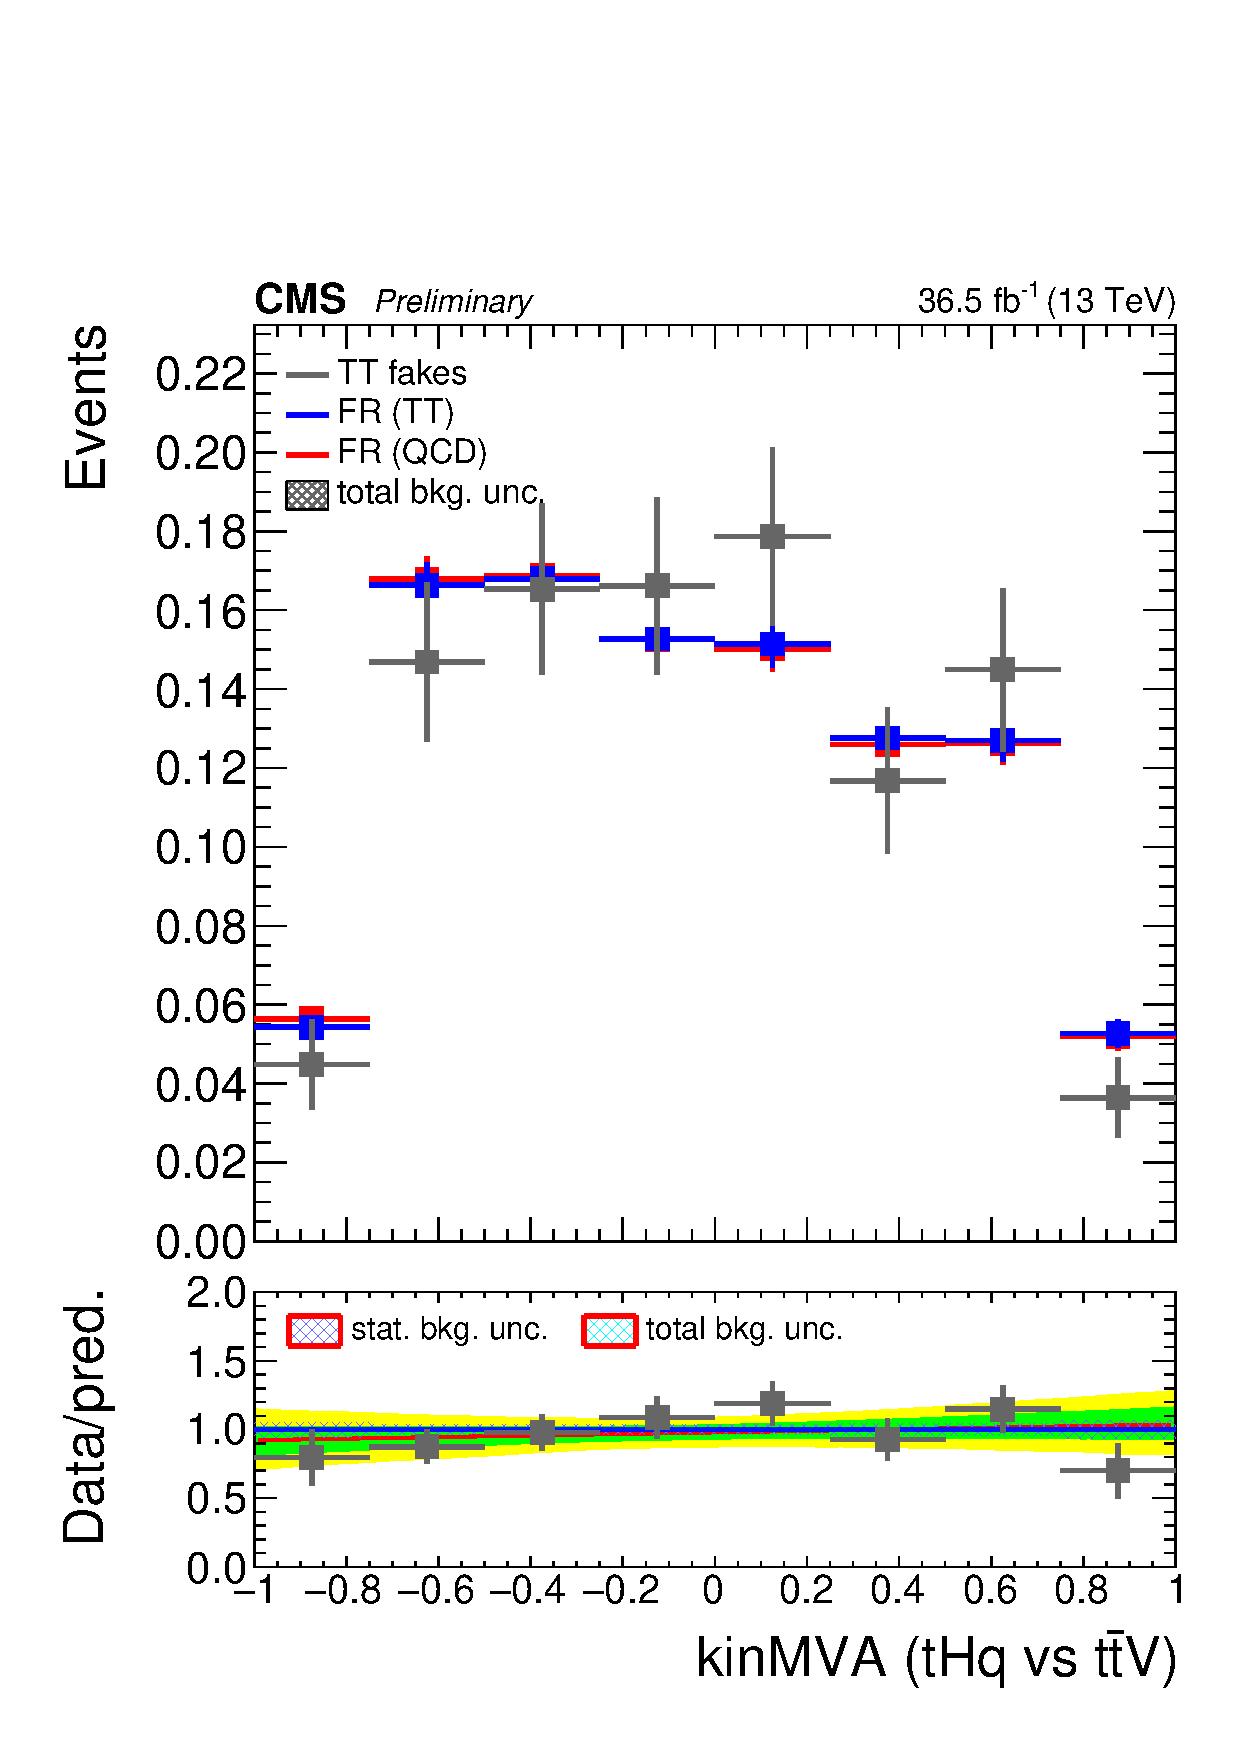
\includegraphics[width=0.245\textwidth]{figures/FR_closures/thqMVA_ttv_2lss_ee_shape.pdf}\\ 
\caption{BDT outputs comparing \ttbar\ MC to a fake-rate prediction using fake rates measured in QCD MC.\@ Agreement in normalization is estimated from the left two plots, shape disagreement is estimated from the right two (normalized) plots. Same-sign \ee\ selection.} 
\label{fig:frclosure_2lss_ee}
\end{figure} 

\begin{figure}[htb]
 \centering
 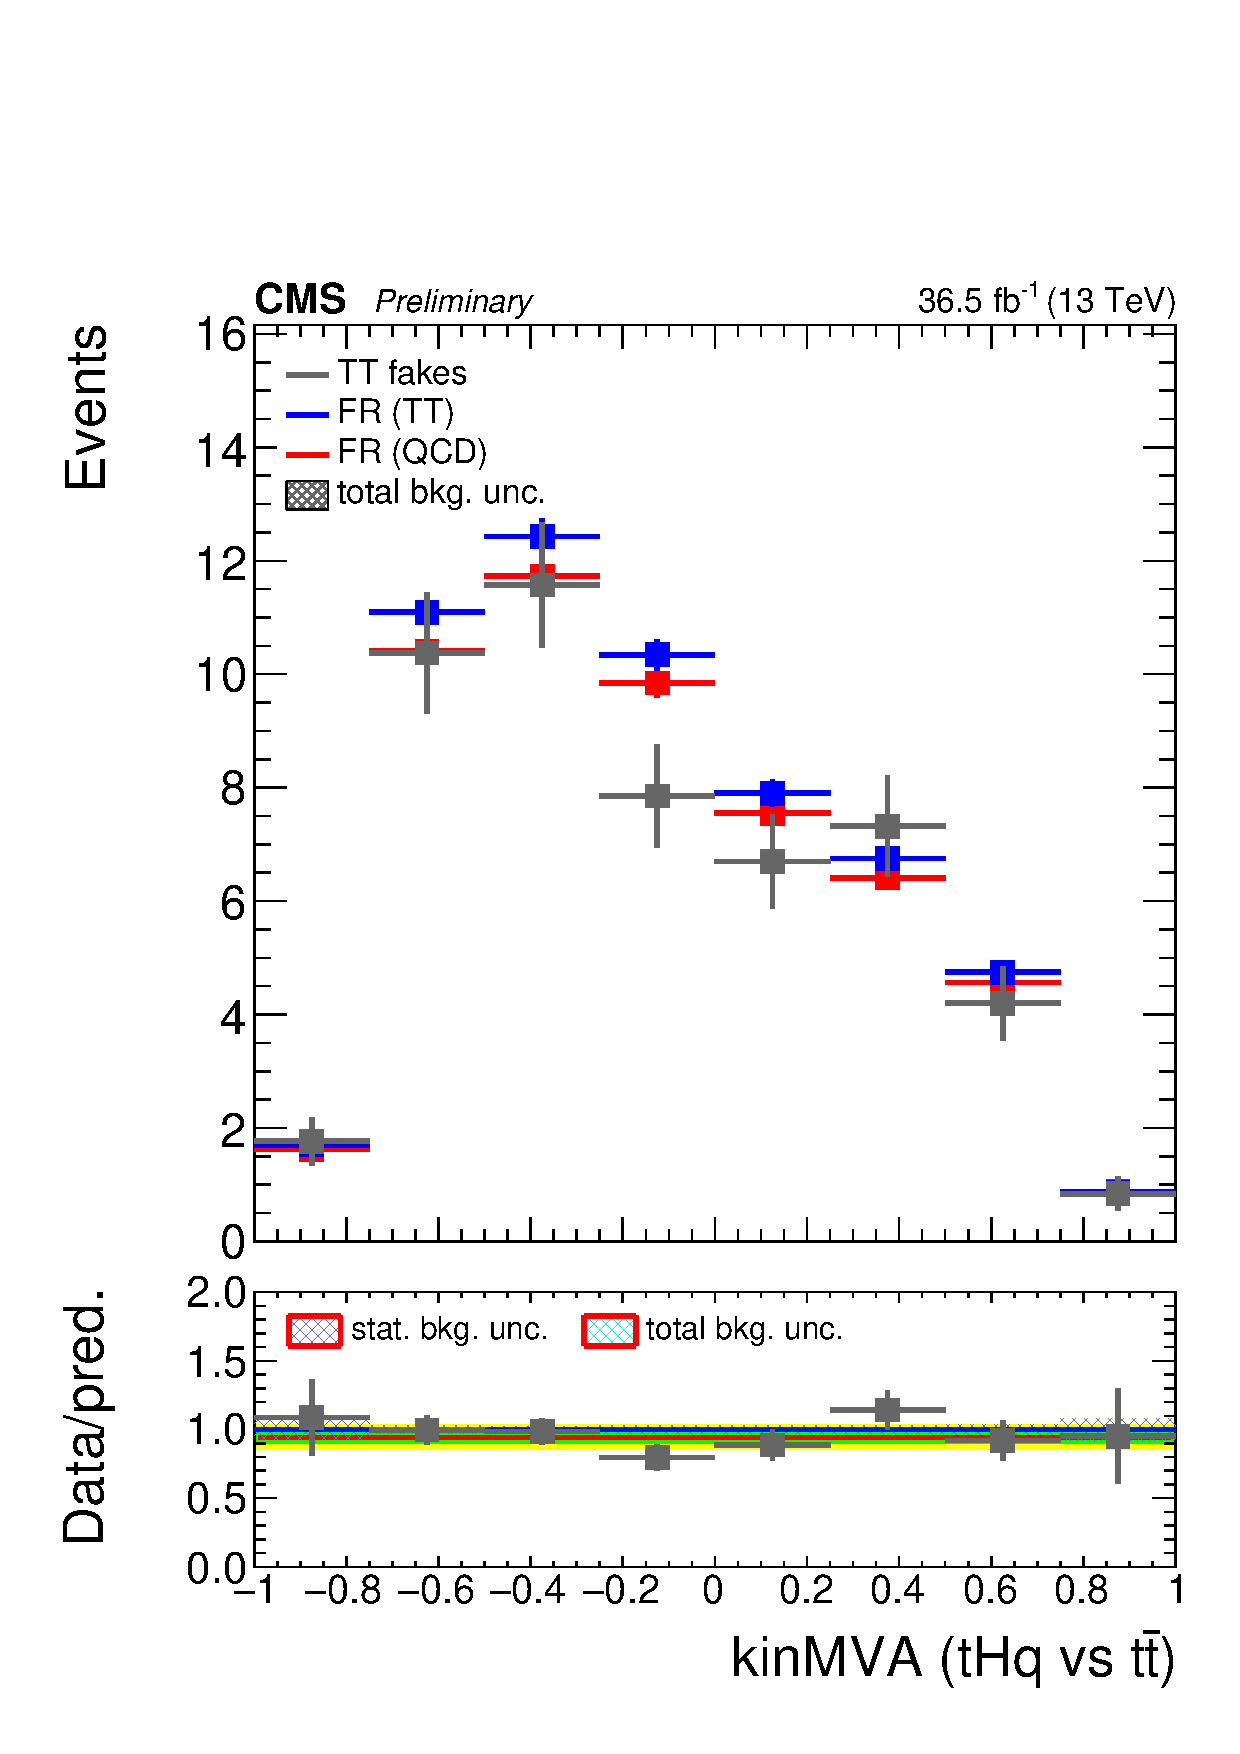
\includegraphics[width=0.245\textwidth]{figures/FR_closures/thqMVA_tt_2lss_em_elfake_norm.pdf} 
 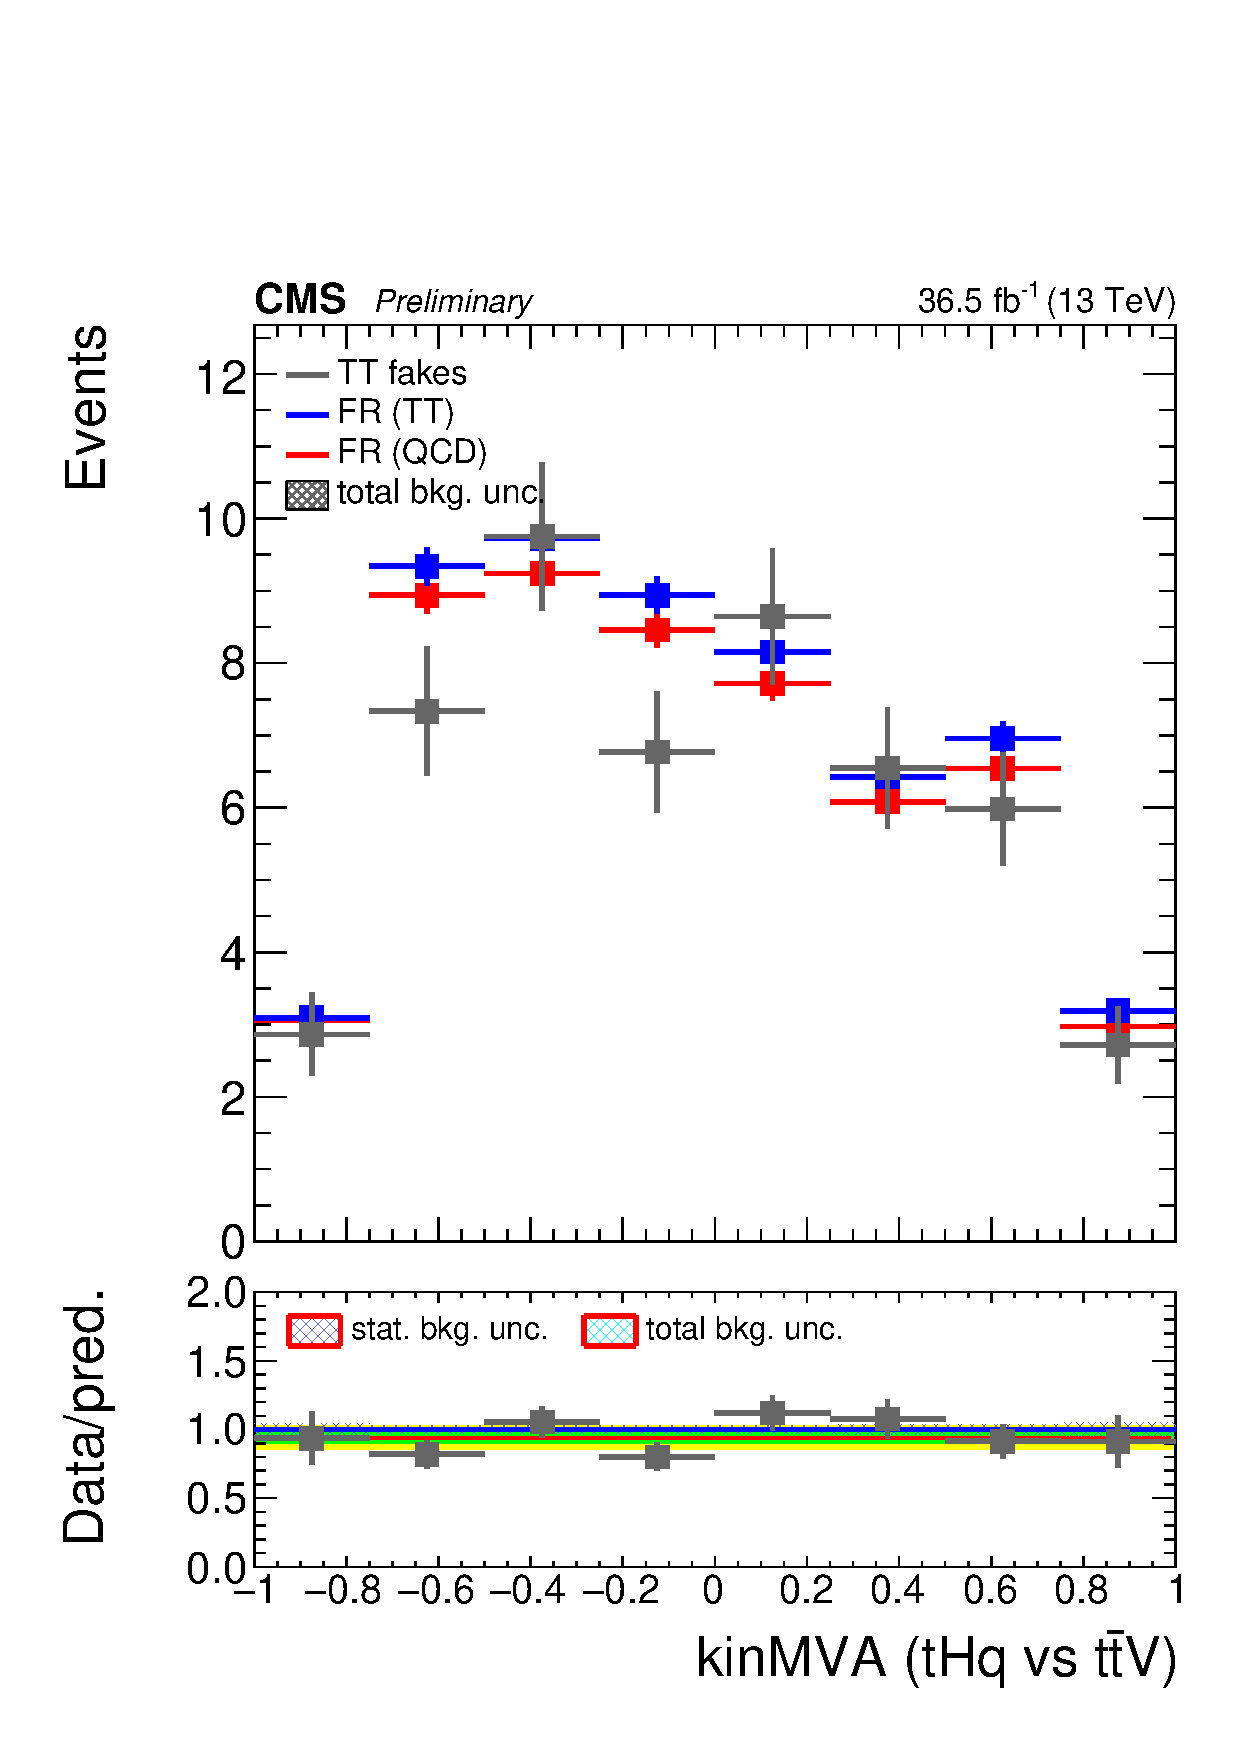
\includegraphics[width=0.245\textwidth]{figures/FR_closures/thqMVA_ttv_2lss_em_elfake_norm.pdf} 
 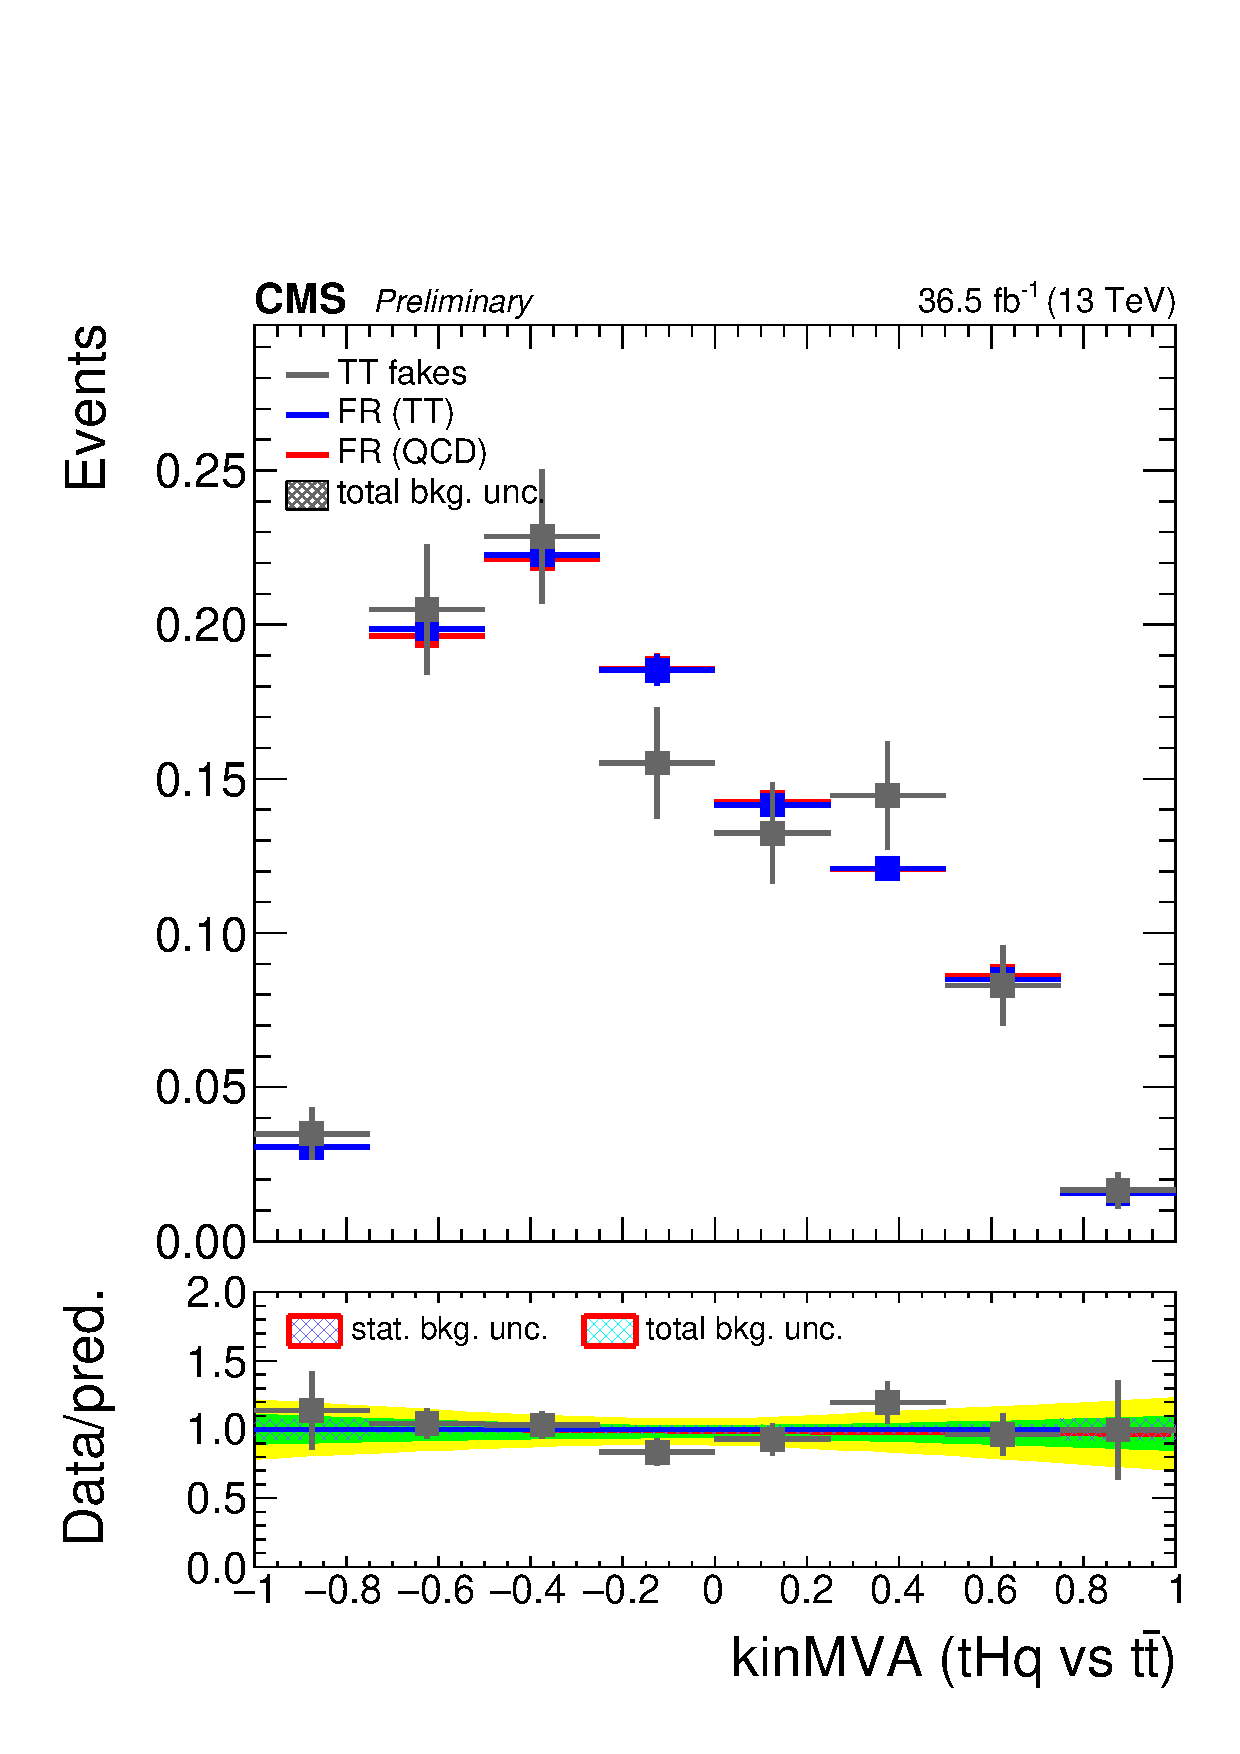
\includegraphics[width=0.245\textwidth]{figures/FR_closures/thqMVA_tt_2lss_em_elfake_shape.pdf} 
 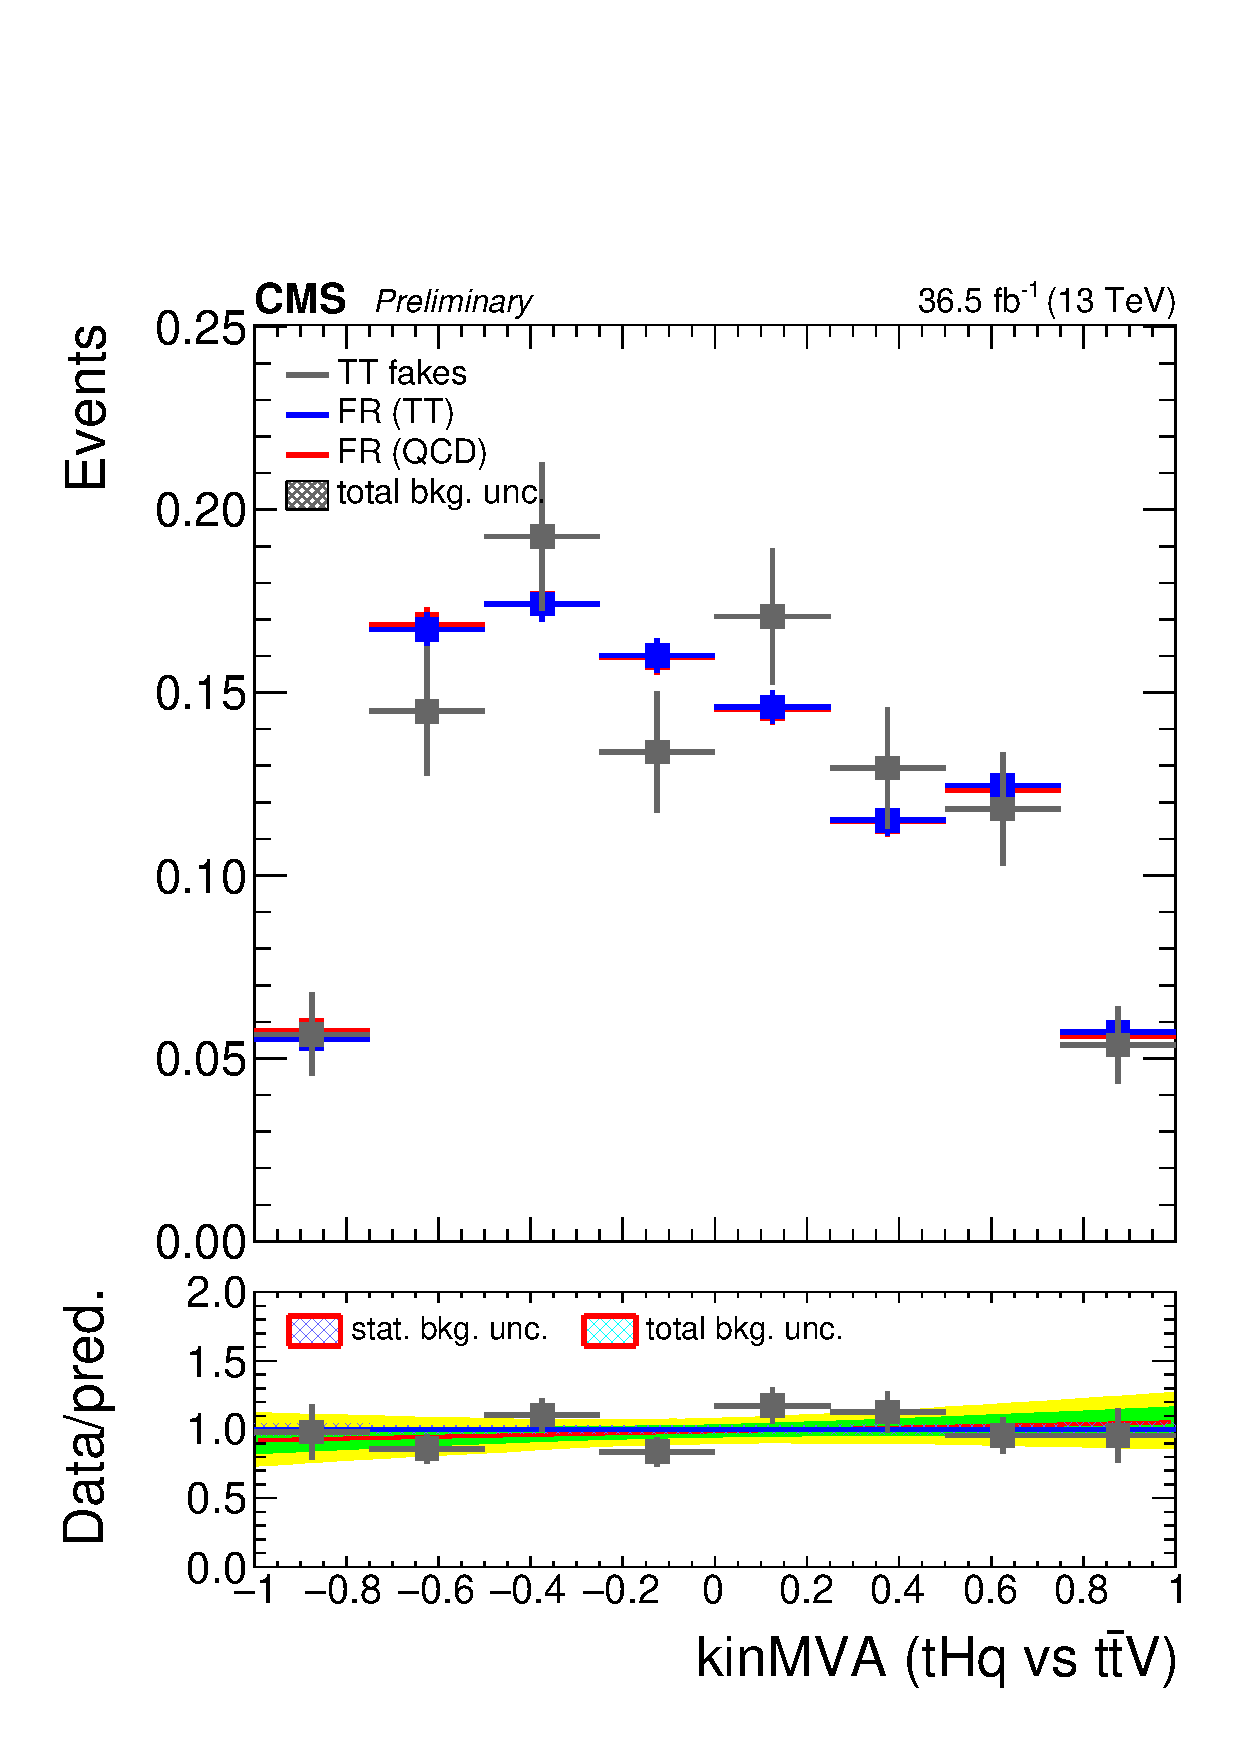
\includegraphics[width=0.245\textwidth]{figures/FR_closures/thqMVA_ttv_2lss_em_elfake_shape.pdf}\\ 
\caption{BDT outputs comparing \ttbar\ MC to a fake-rate prediction using fake rates measured in QCD MC.\@ Agreement in normalization is estimated from the left two plots, shape disagreement is estimated from the right two (normalized) plots. Same-sign \emu\ selection with electron fakes.} 
\label{fig:frclosure_2lss_em_elfake}
\end{figure} 

\begin{figure}[htb]
 \centering
 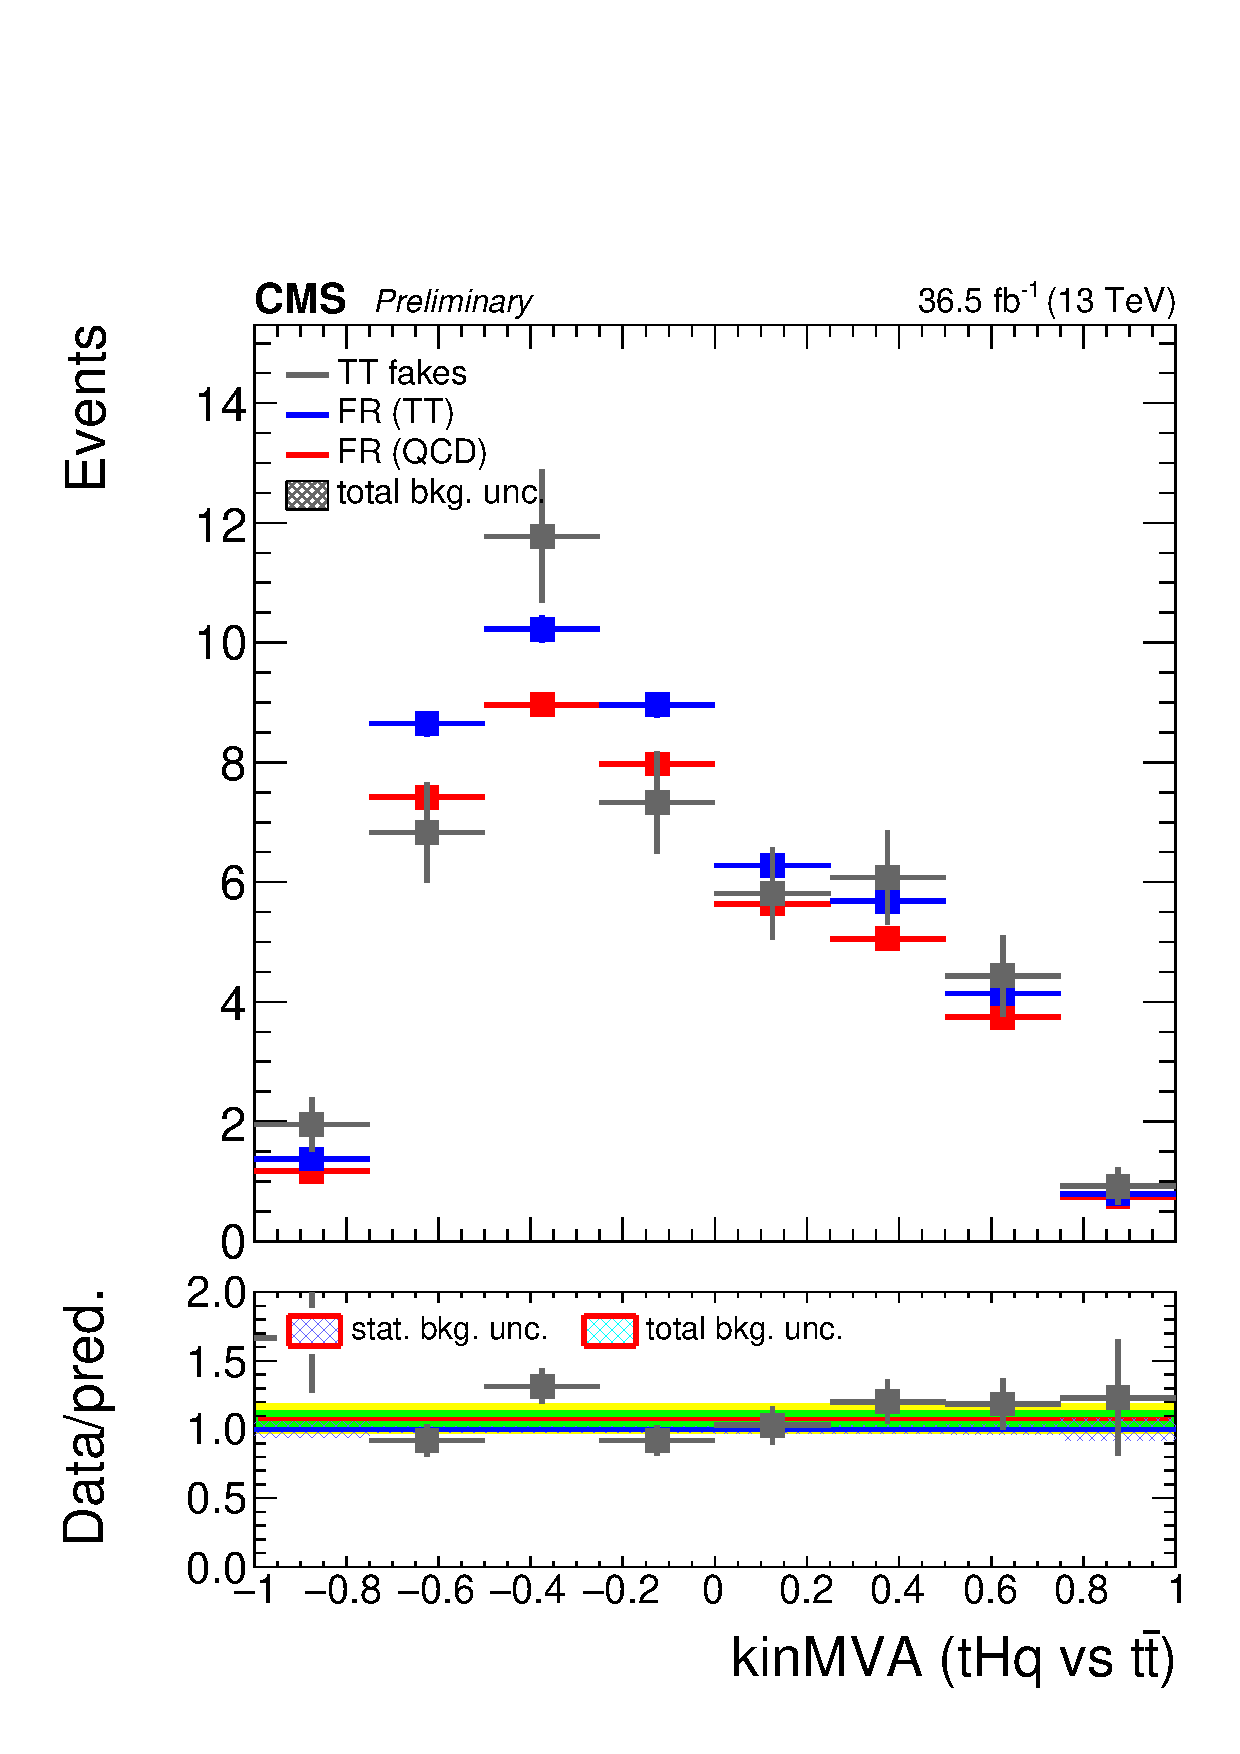
\includegraphics[width=0.245\textwidth]{figures/FR_closures/thqMVA_tt_2lss_em_mufake_norm.pdf} 
 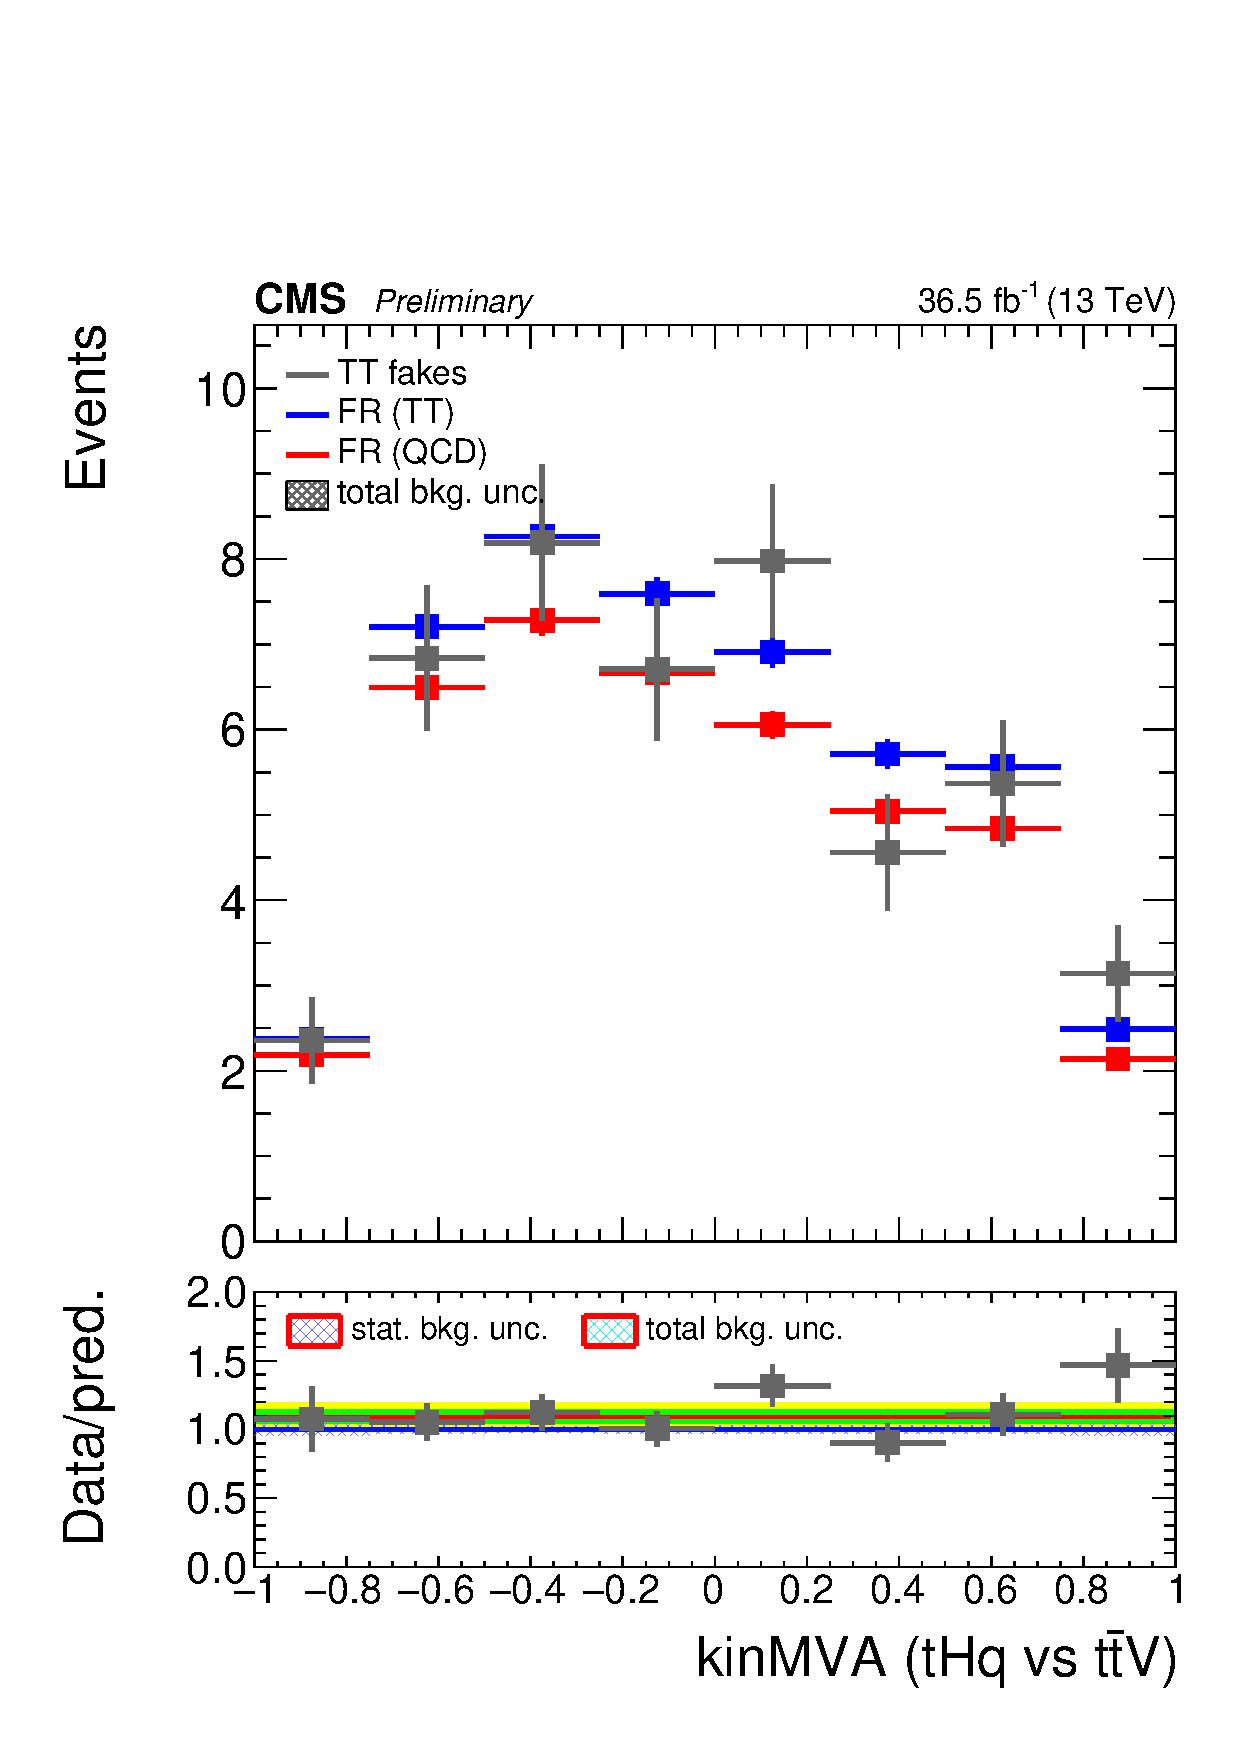
\includegraphics[width=0.245\textwidth]{figures/FR_closures/thqMVA_ttv_2lss_em_mufake_norm.pdf} 
 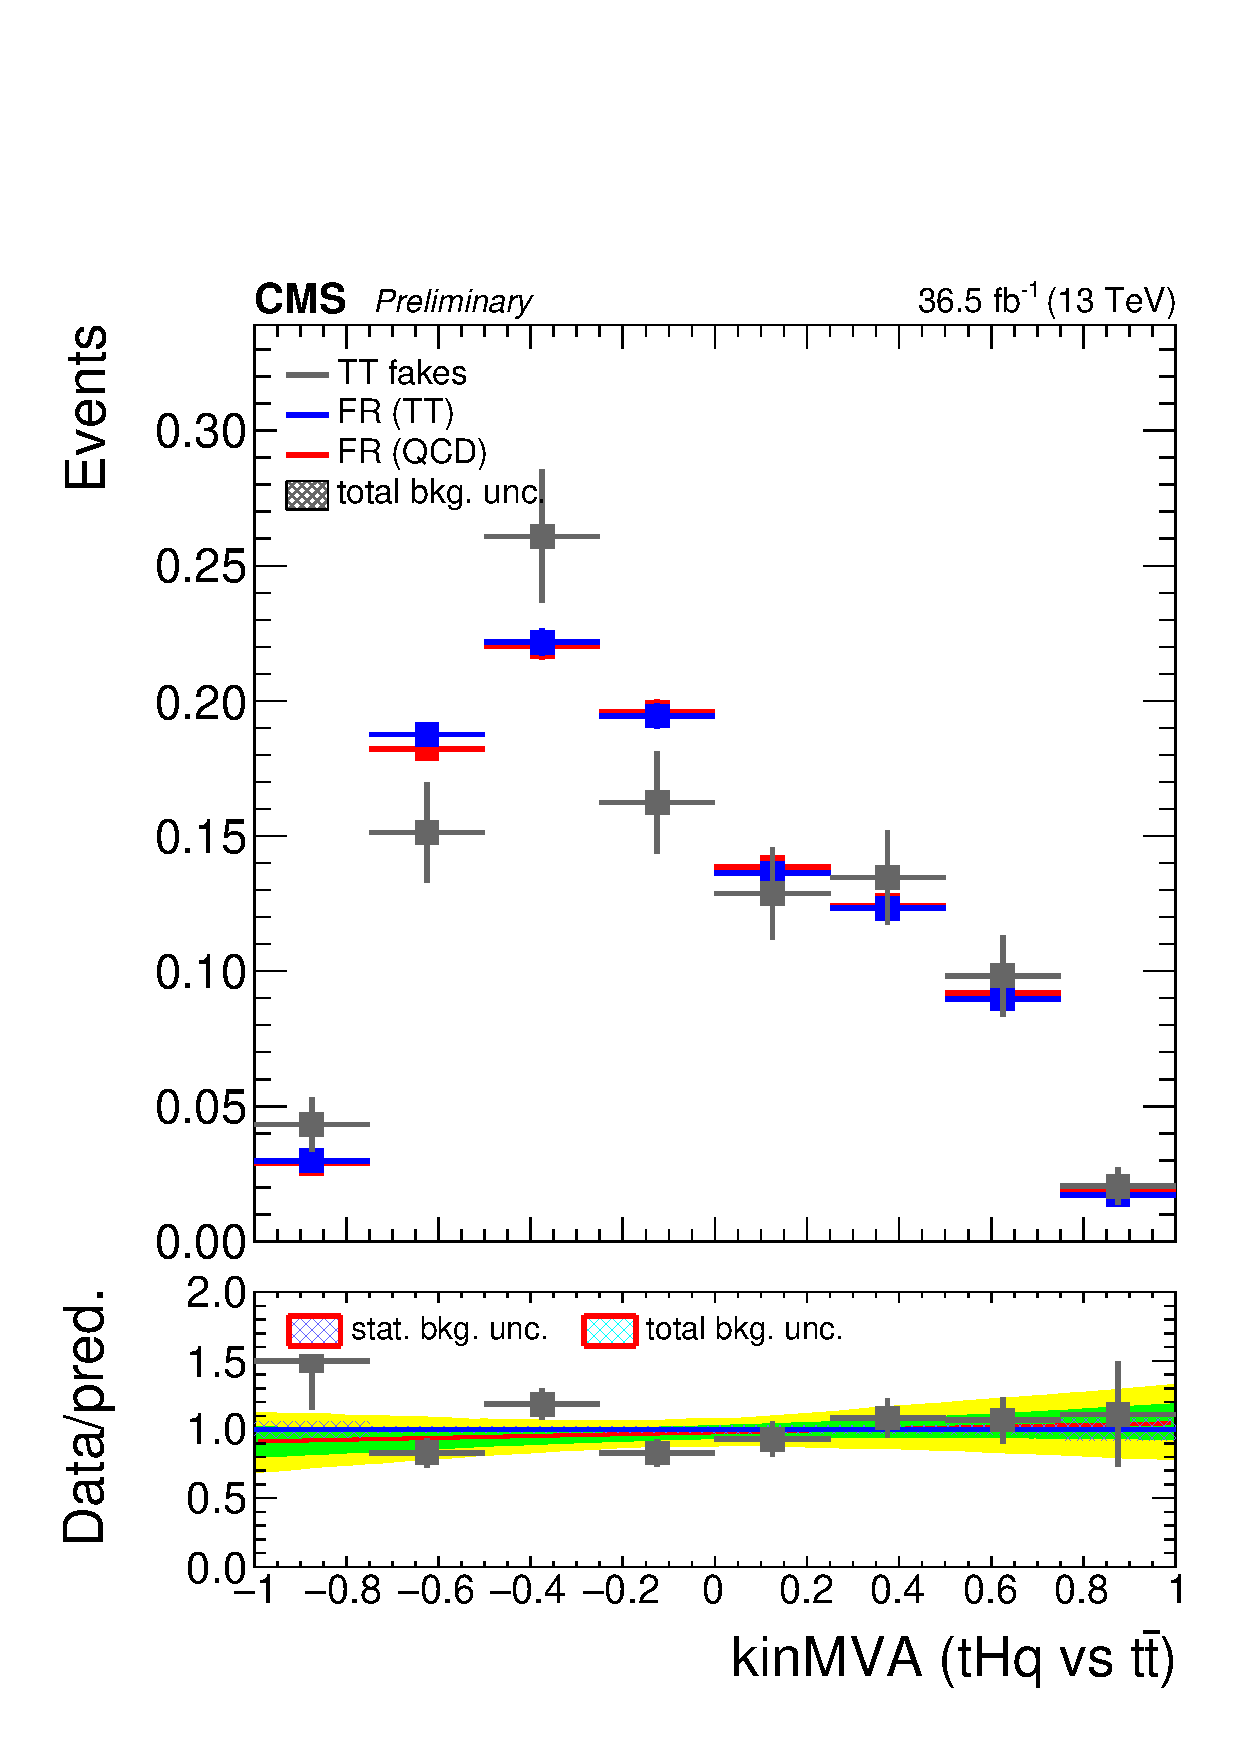
\includegraphics[width=0.245\textwidth]{figures/FR_closures/thqMVA_tt_2lss_em_mufake_shape.pdf} 
 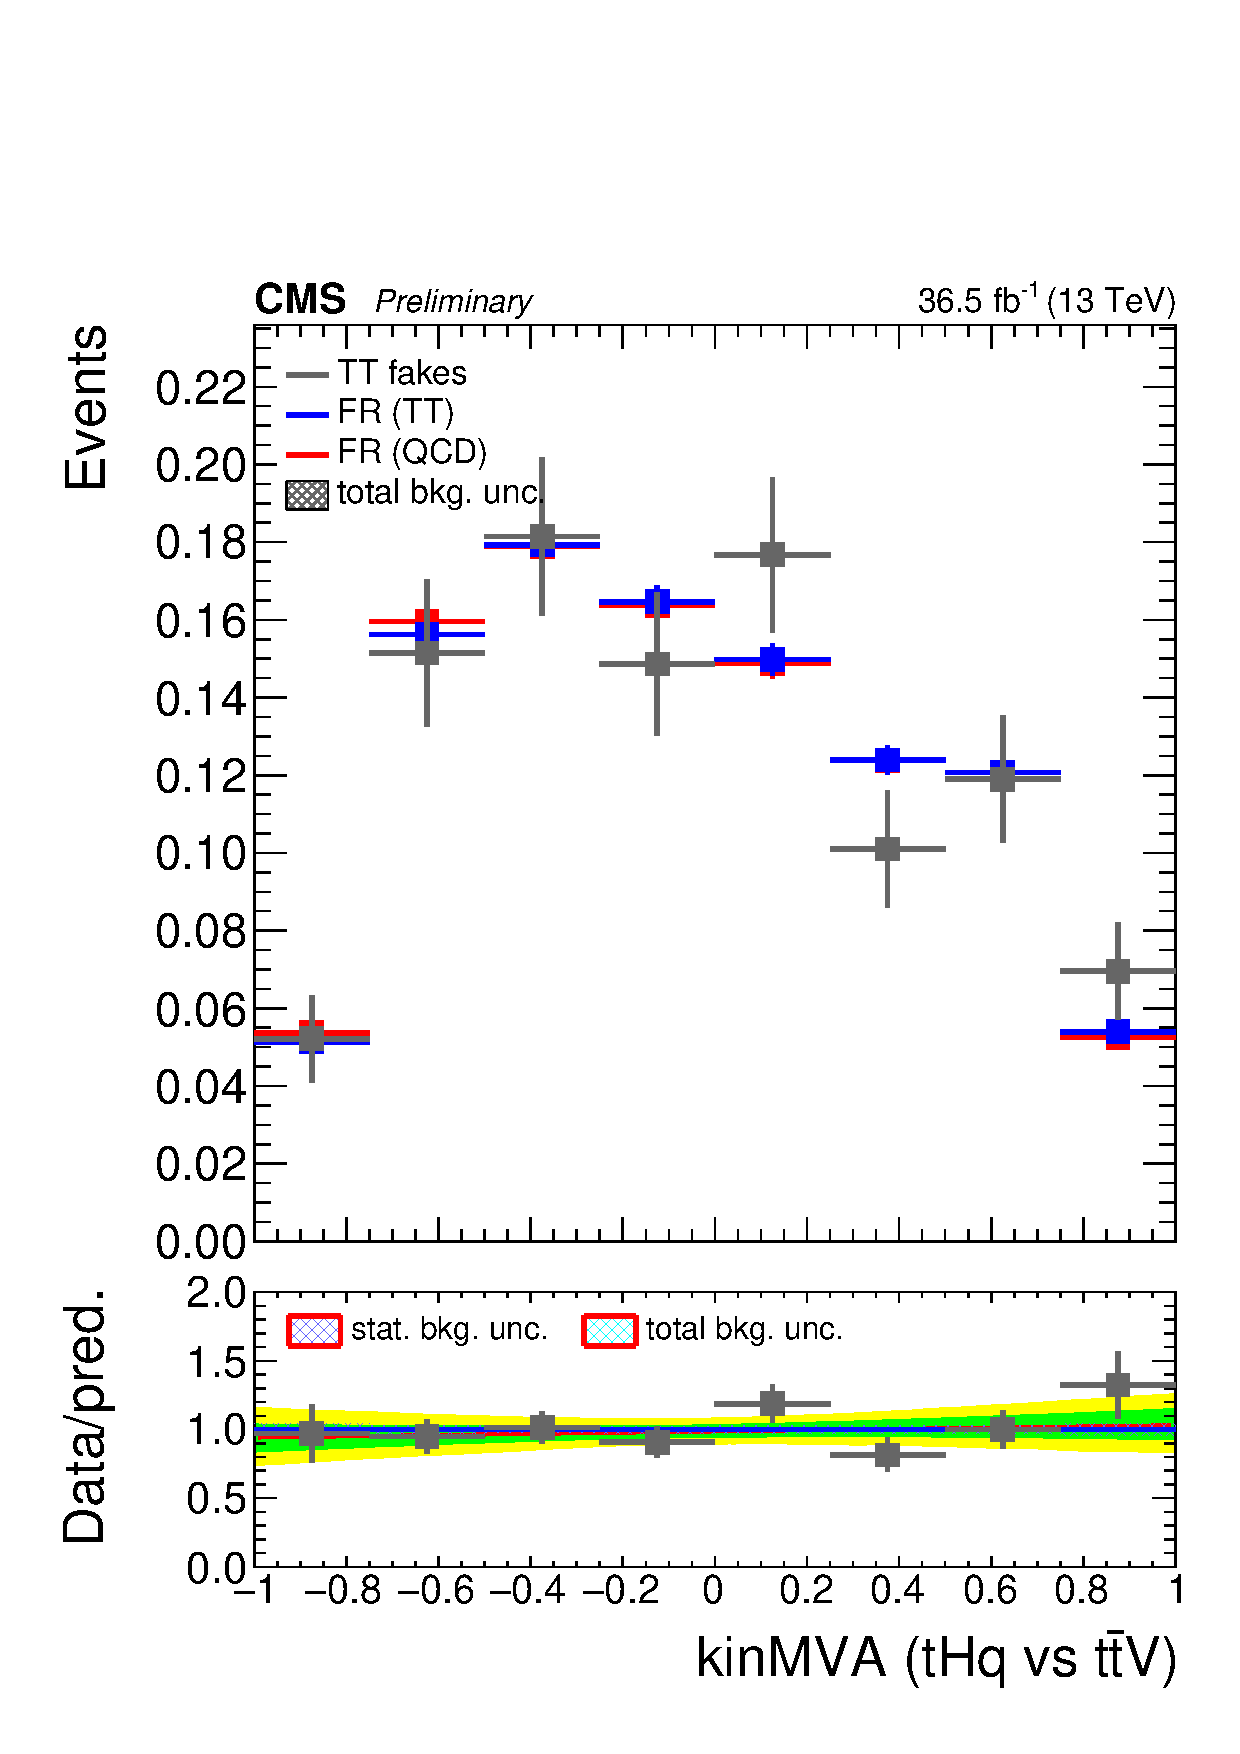
\includegraphics[width=0.245\textwidth]{figures/FR_closures/thqMVA_ttv_2lss_em_mufake_shape.pdf}\\ 
\caption{BDT outputs comparing \ttbar\ MC to a fake-rate prediction using fake rates measured in QCD MC.\@ Agreement in normalization is estimated from the left two plots, shape disagreement is estimated from the right two (normalized) plots. Same-sign \emu\ selection with muon fakes.} 
\label{fig:frclosure_2lss_em_mufake}
\end{figure} 

\begin{figure}[htb]
 \centering
 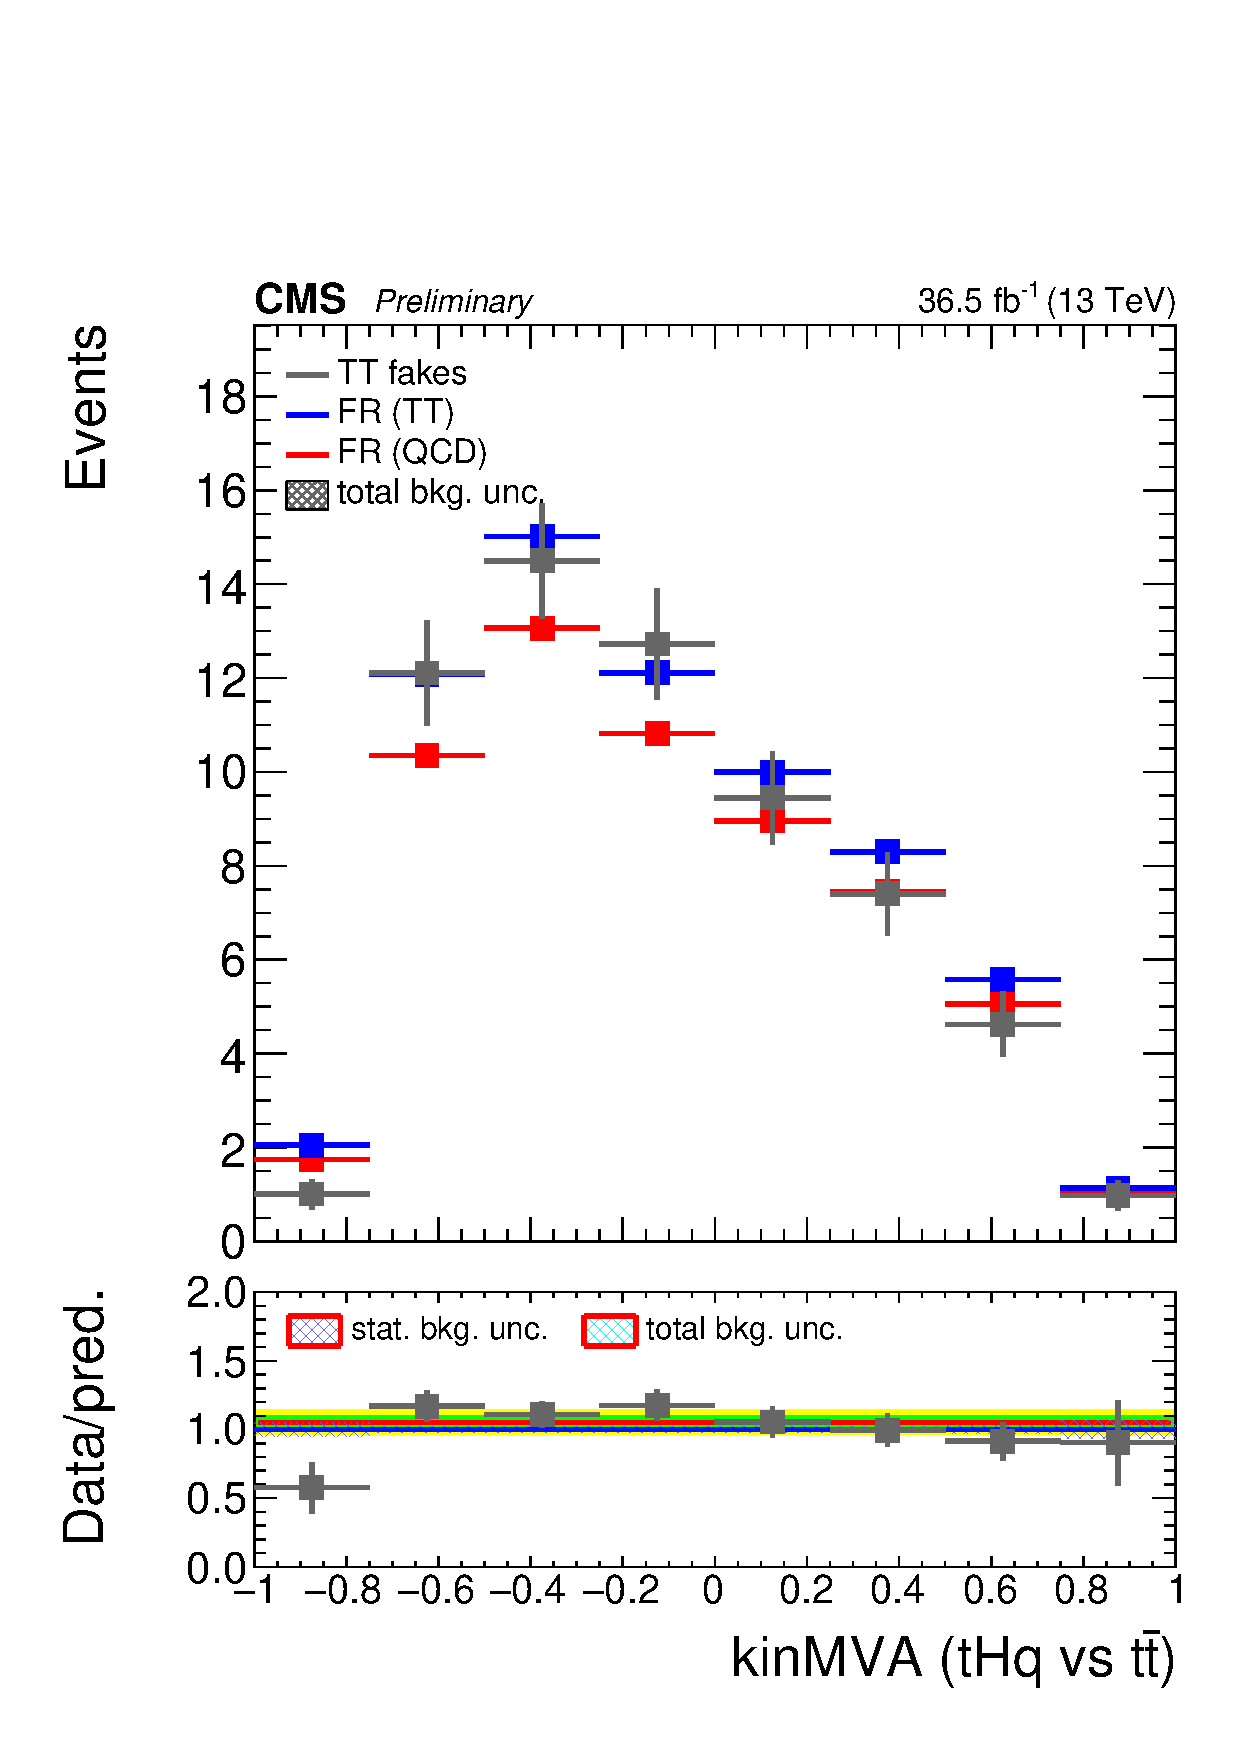
\includegraphics[width=0.245\textwidth]{figures/FR_closures/thqMVA_tt_2lss_mm_norm.pdf} 
 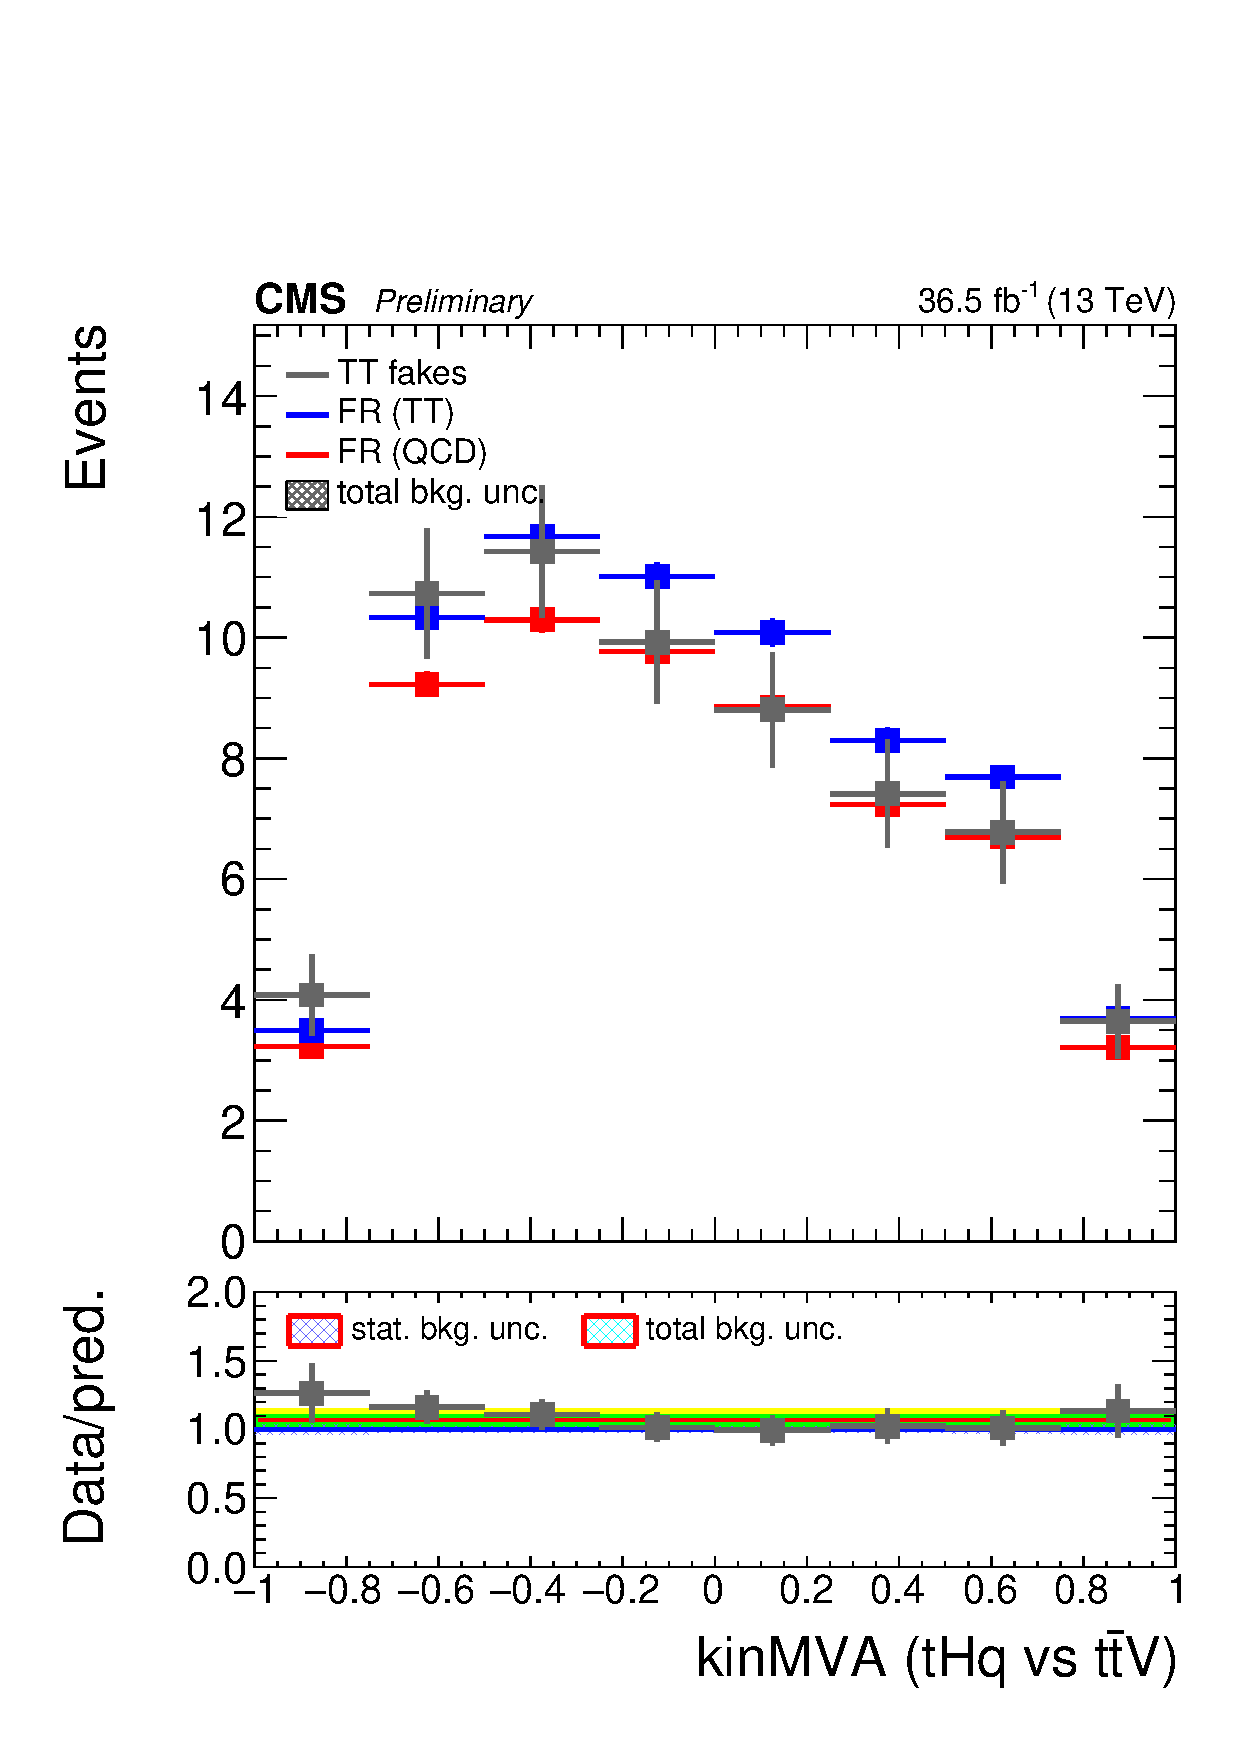
\includegraphics[width=0.245\textwidth]{figures/FR_closures/thqMVA_ttv_2lss_mm_norm.pdf} 
 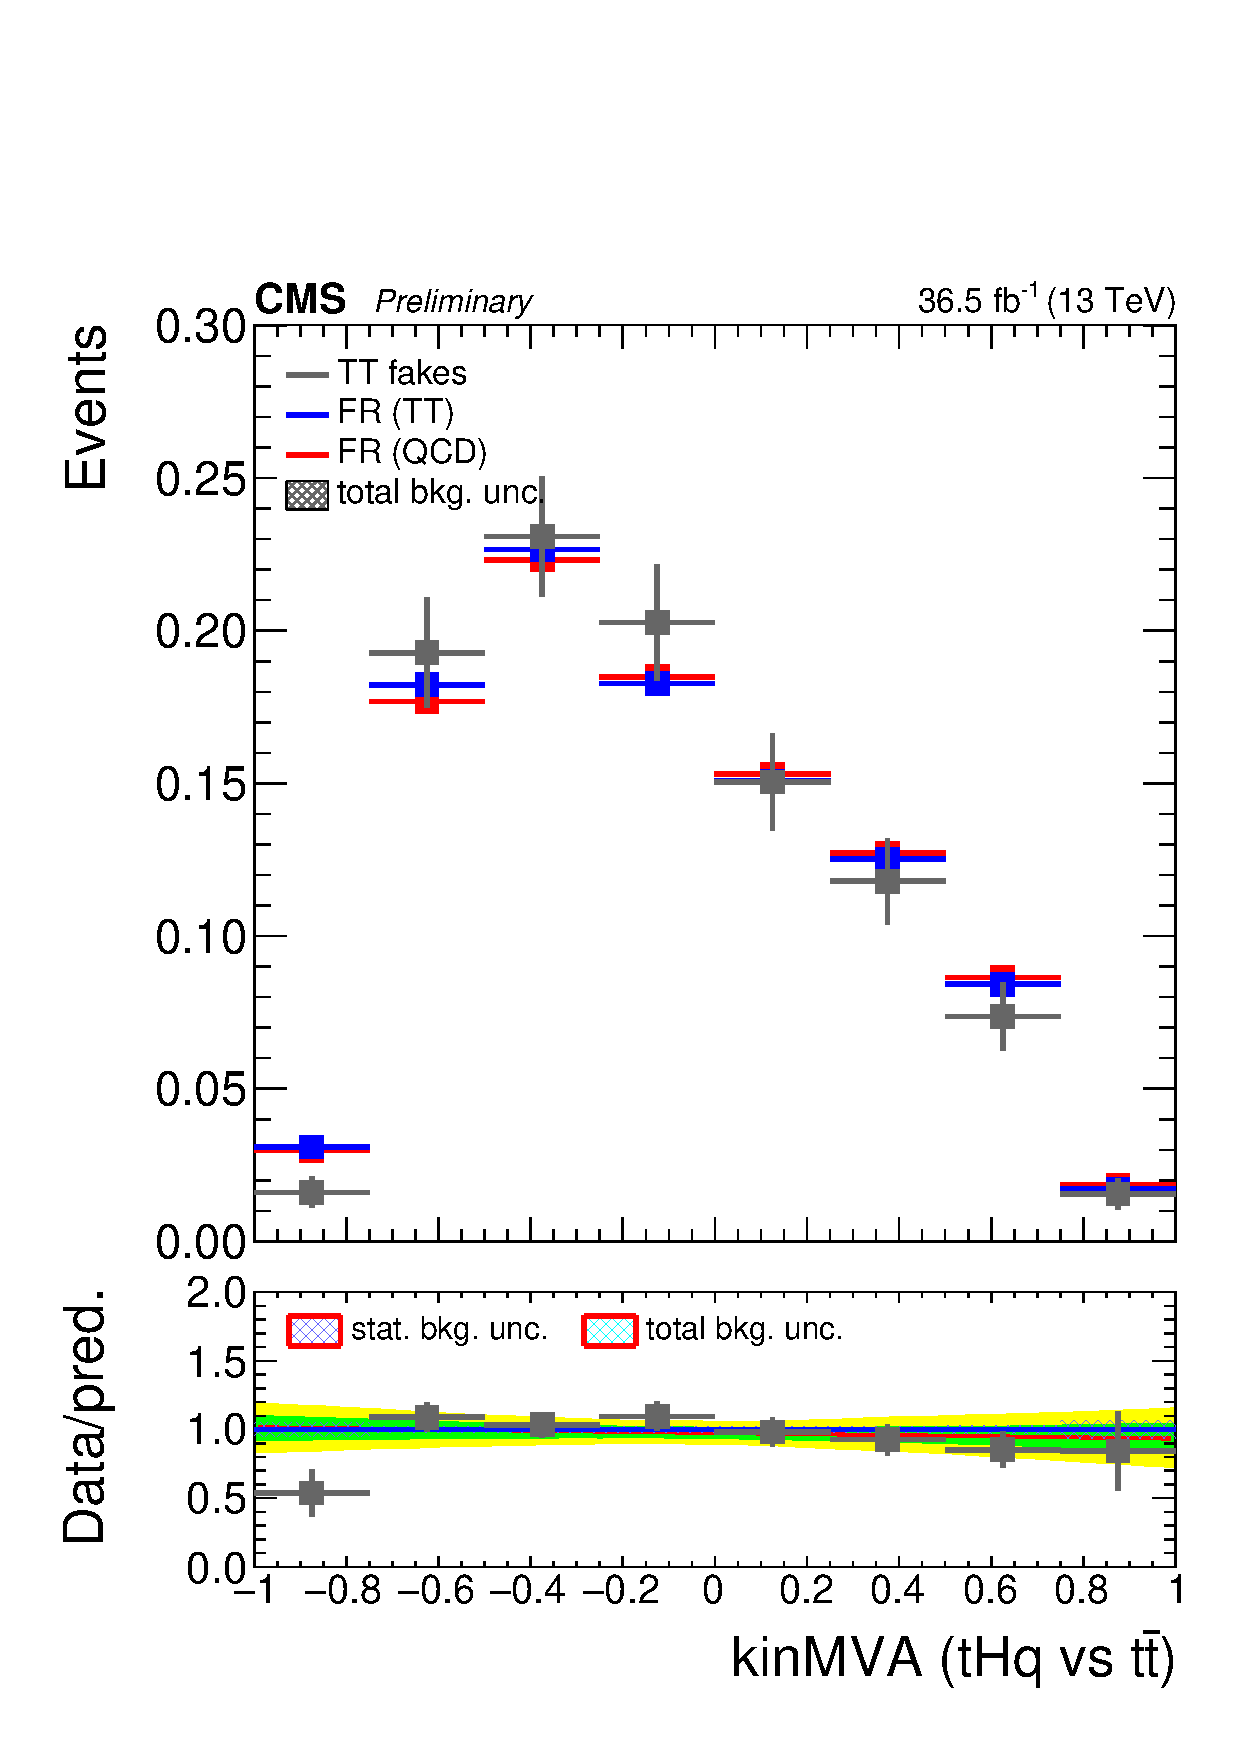
\includegraphics[width=0.245\textwidth]{figures/FR_closures/thqMVA_tt_2lss_mm_shape.pdf} 
 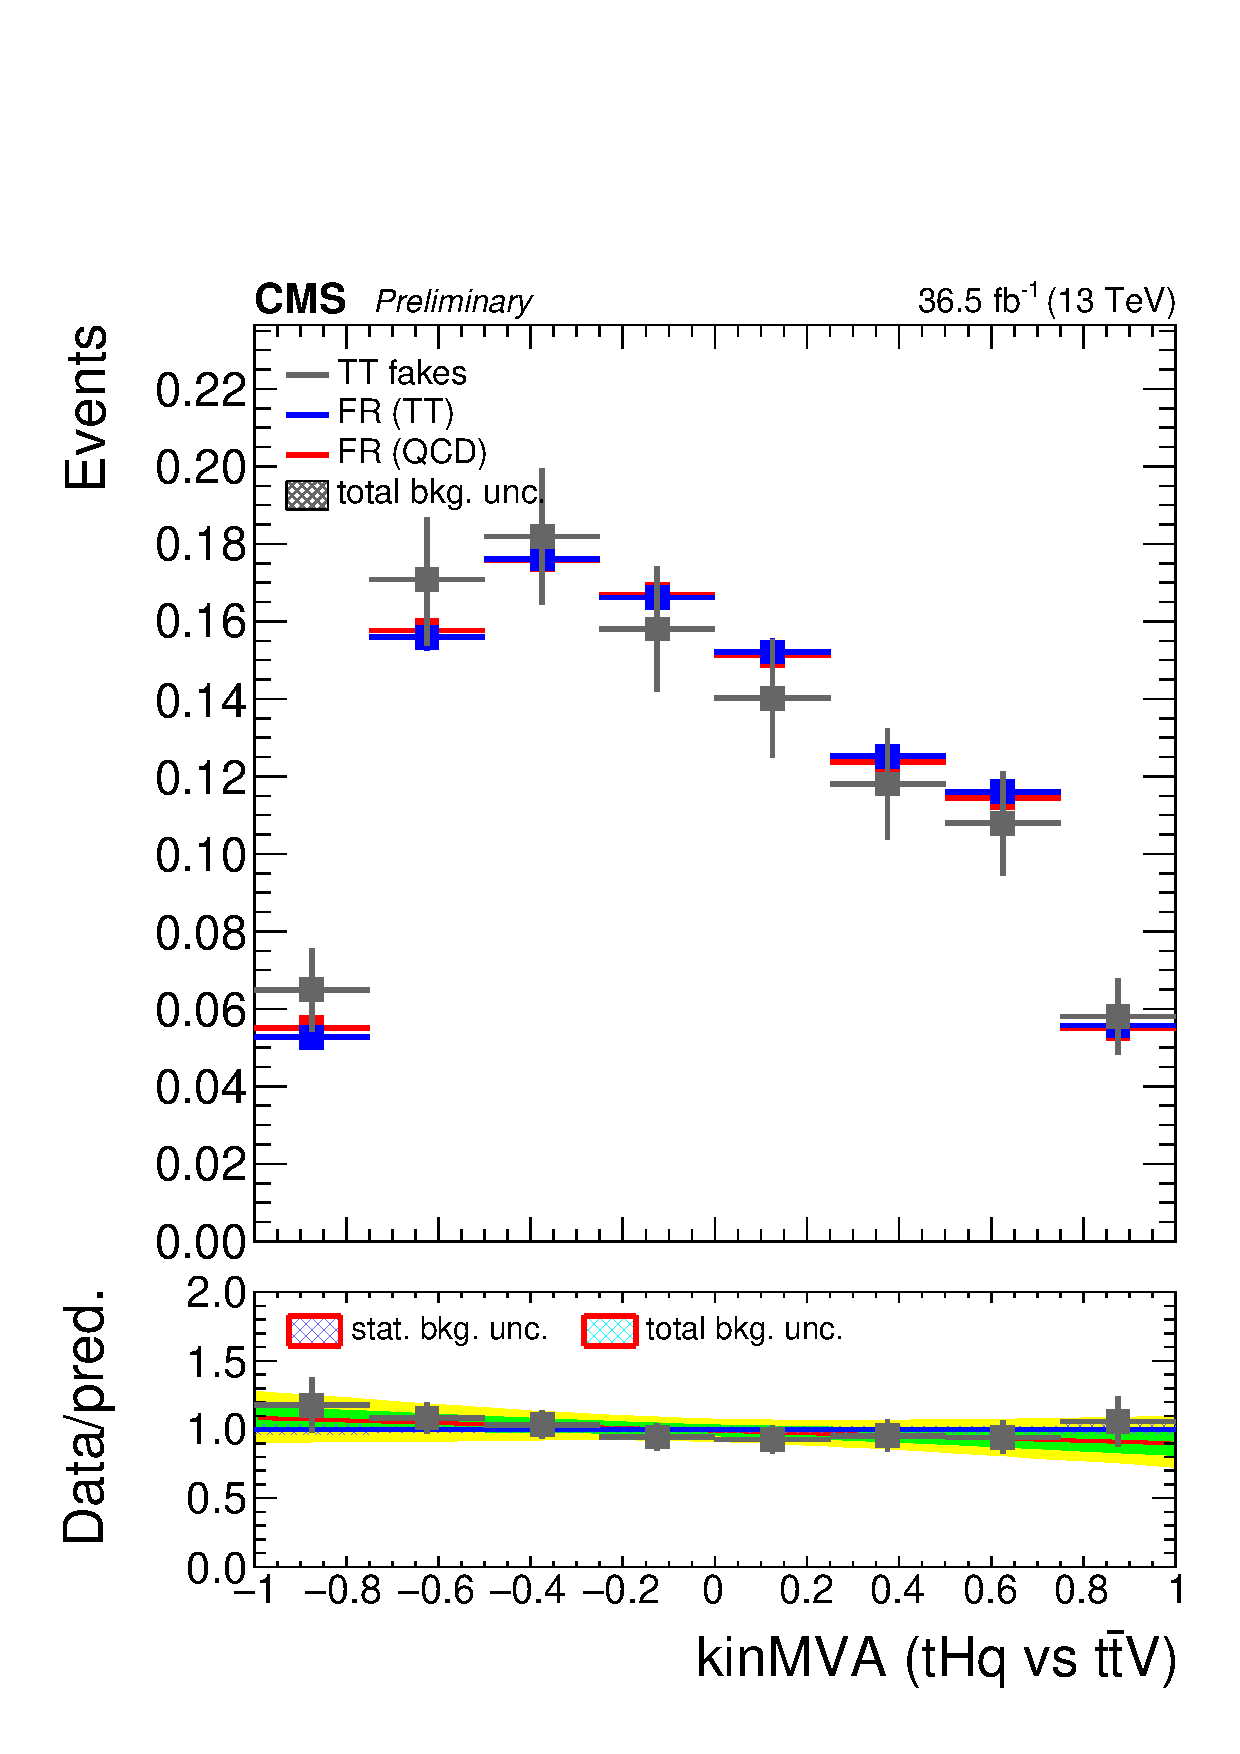
\includegraphics[width=0.245\textwidth]{figures/FR_closures/thqMVA_ttv_2lss_mm_shape.pdf} \\
\caption{BDT outputs comparing \ttbar\ MC to a fake-rate prediction using fake rates measured in QCD MC.\@ Agreement in normalization is estimated from the left two plots, shape disagreement is estimated from the right two (normalized) plots. Same-sign \mumu\ selection.} 
\label{fig:frclosure_2lss_mm}
\end{figure} 

\begin{figure}[htb]
 \centering
 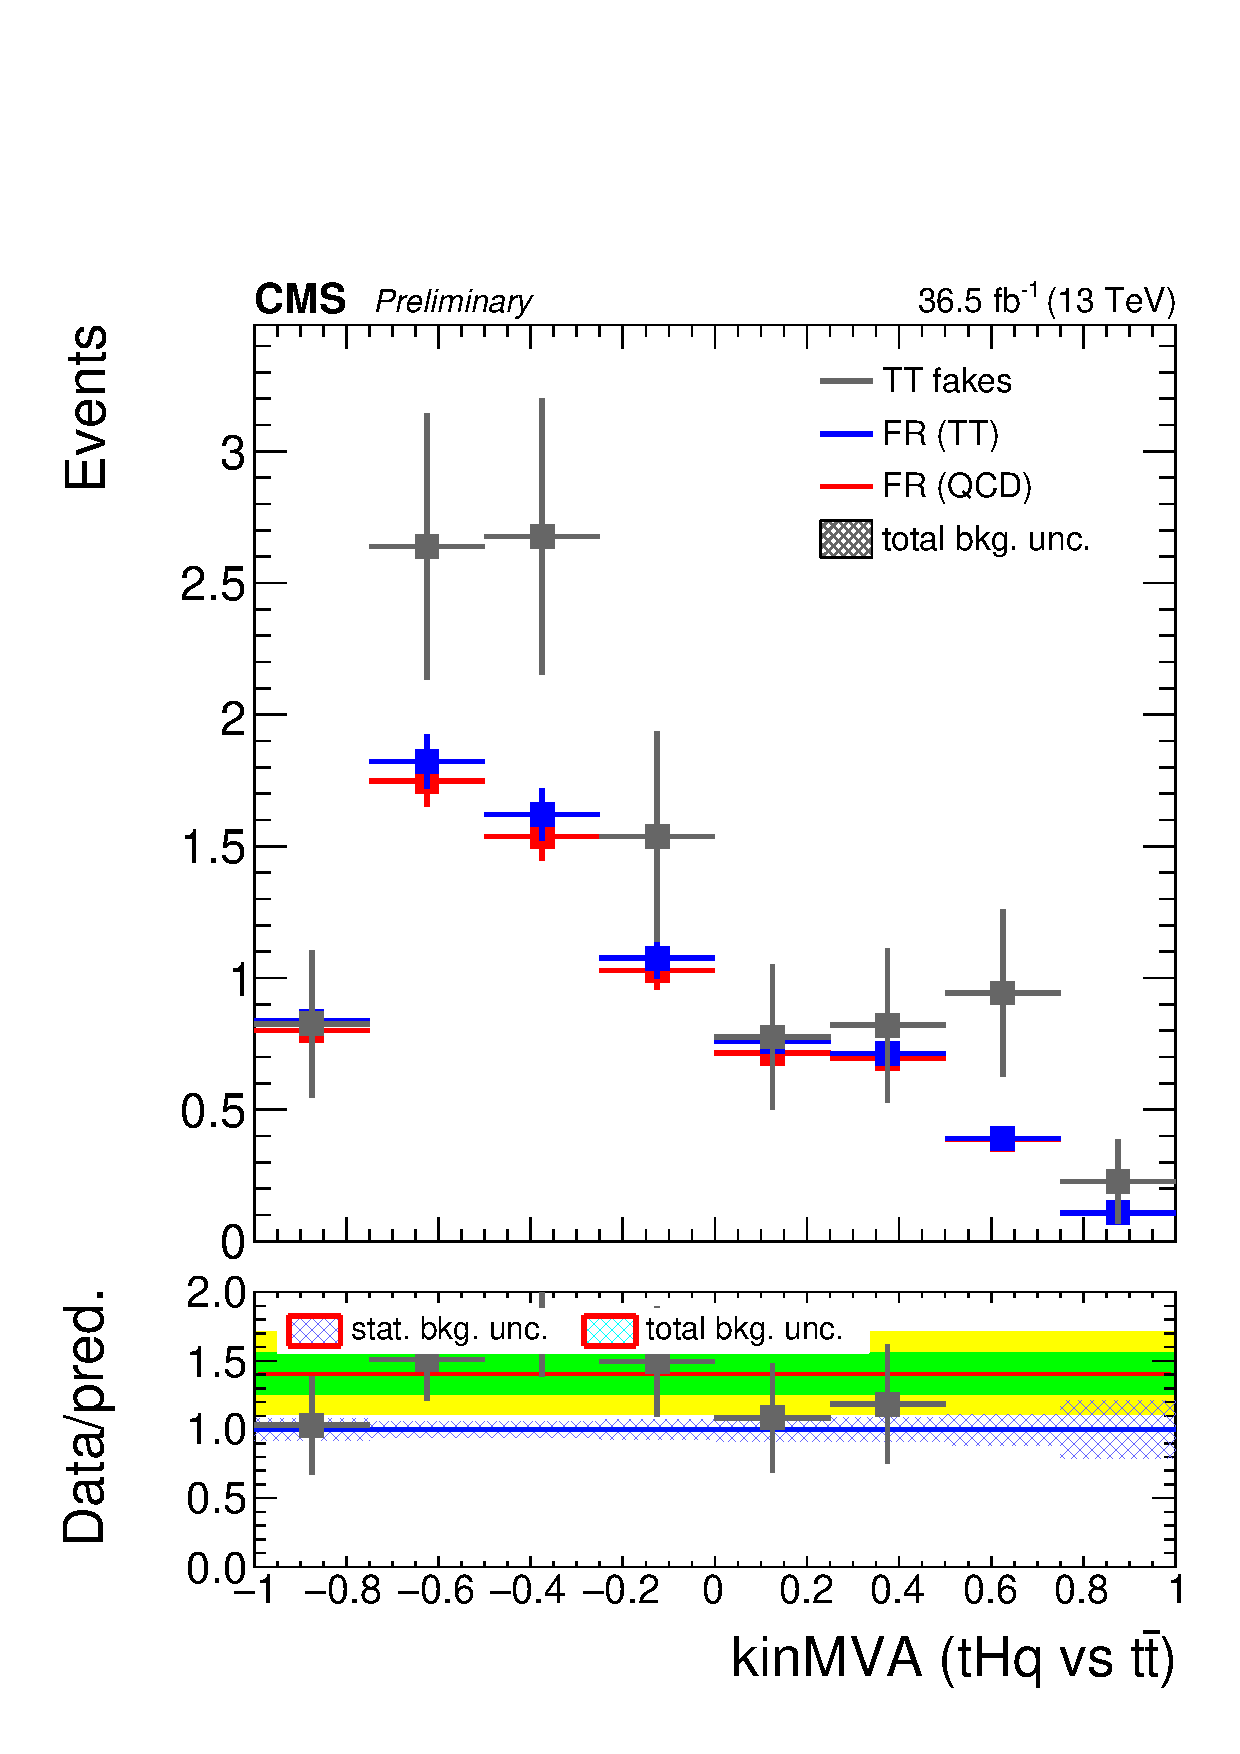
\includegraphics[width=0.245\textwidth]{figures/FR_closures/thqMVA_tt_3l_elfake_norm.pdf} 
 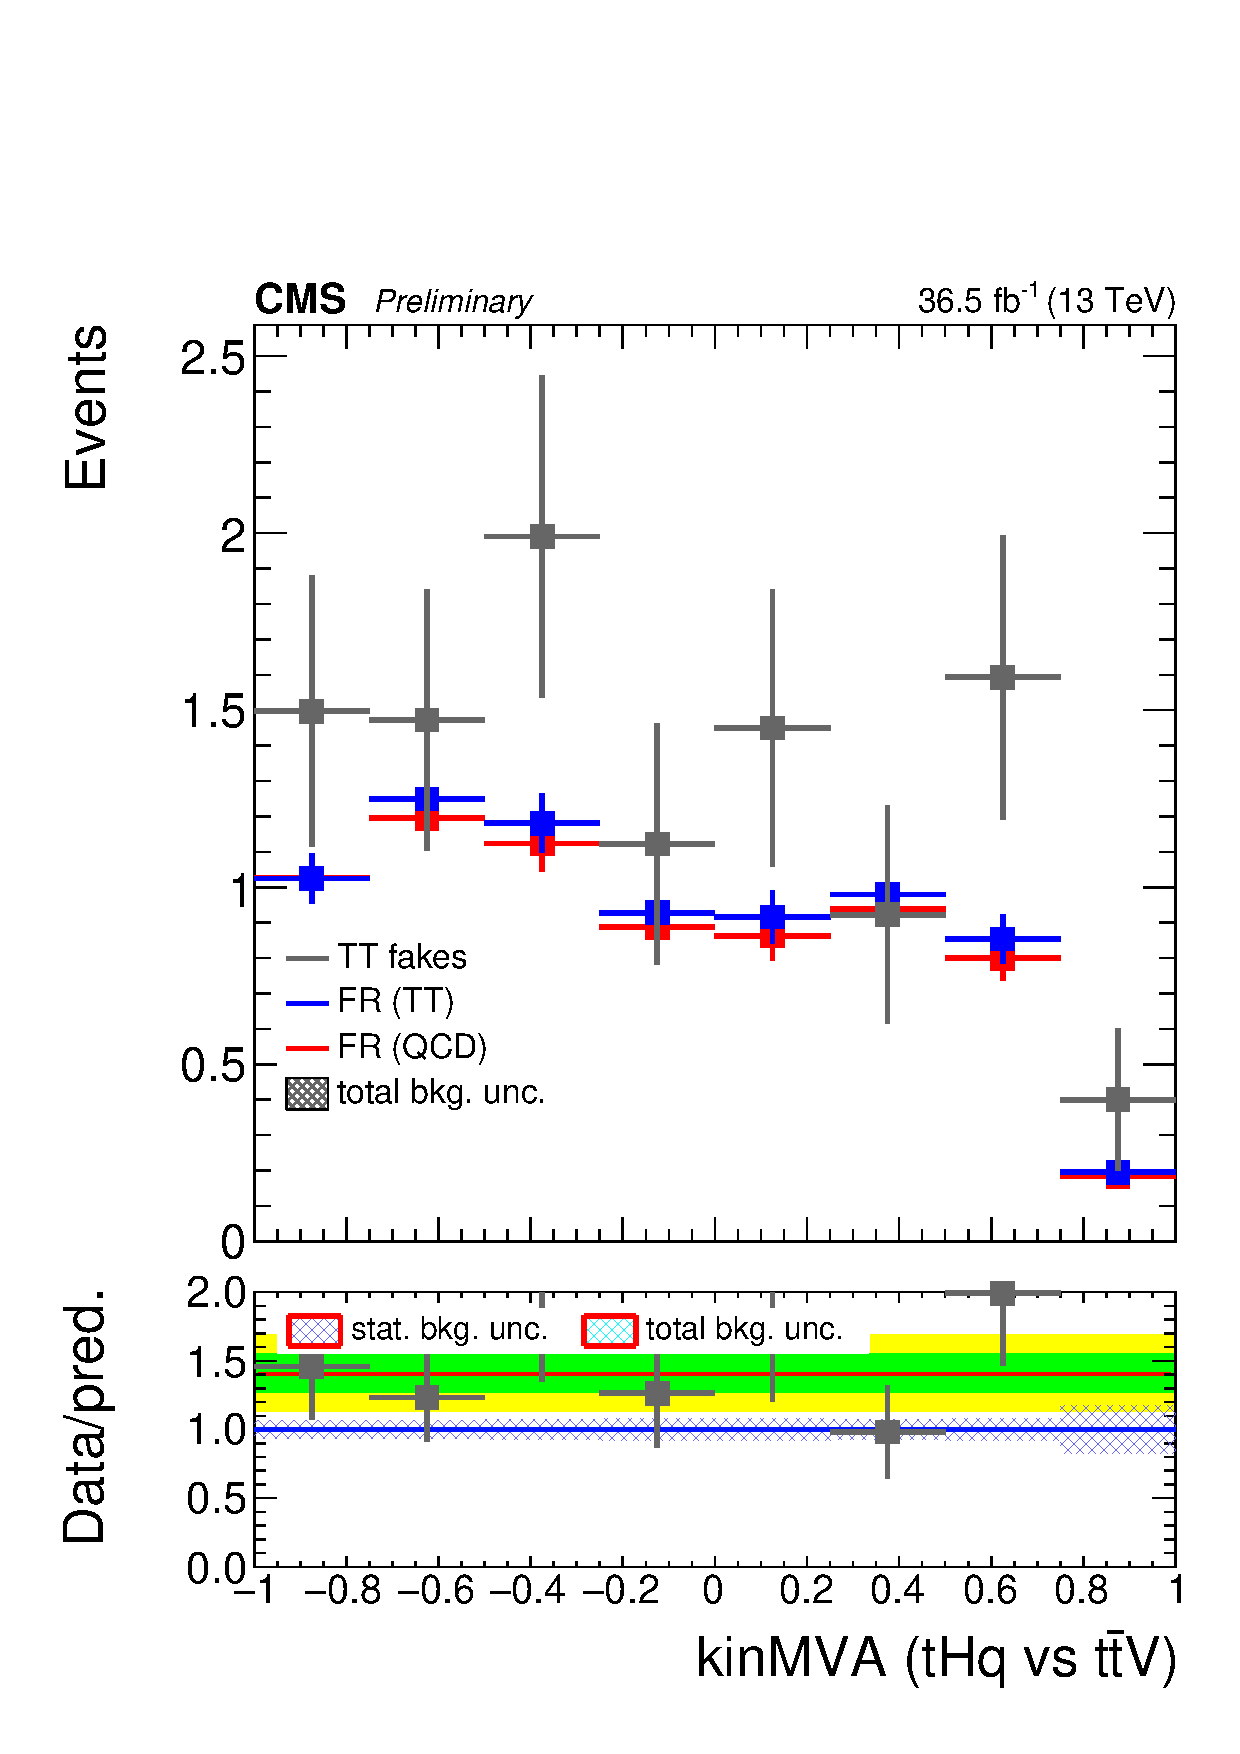
\includegraphics[width=0.245\textwidth]{figures/FR_closures/thqMVA_ttv_3l_elfake_norm.pdf} 
 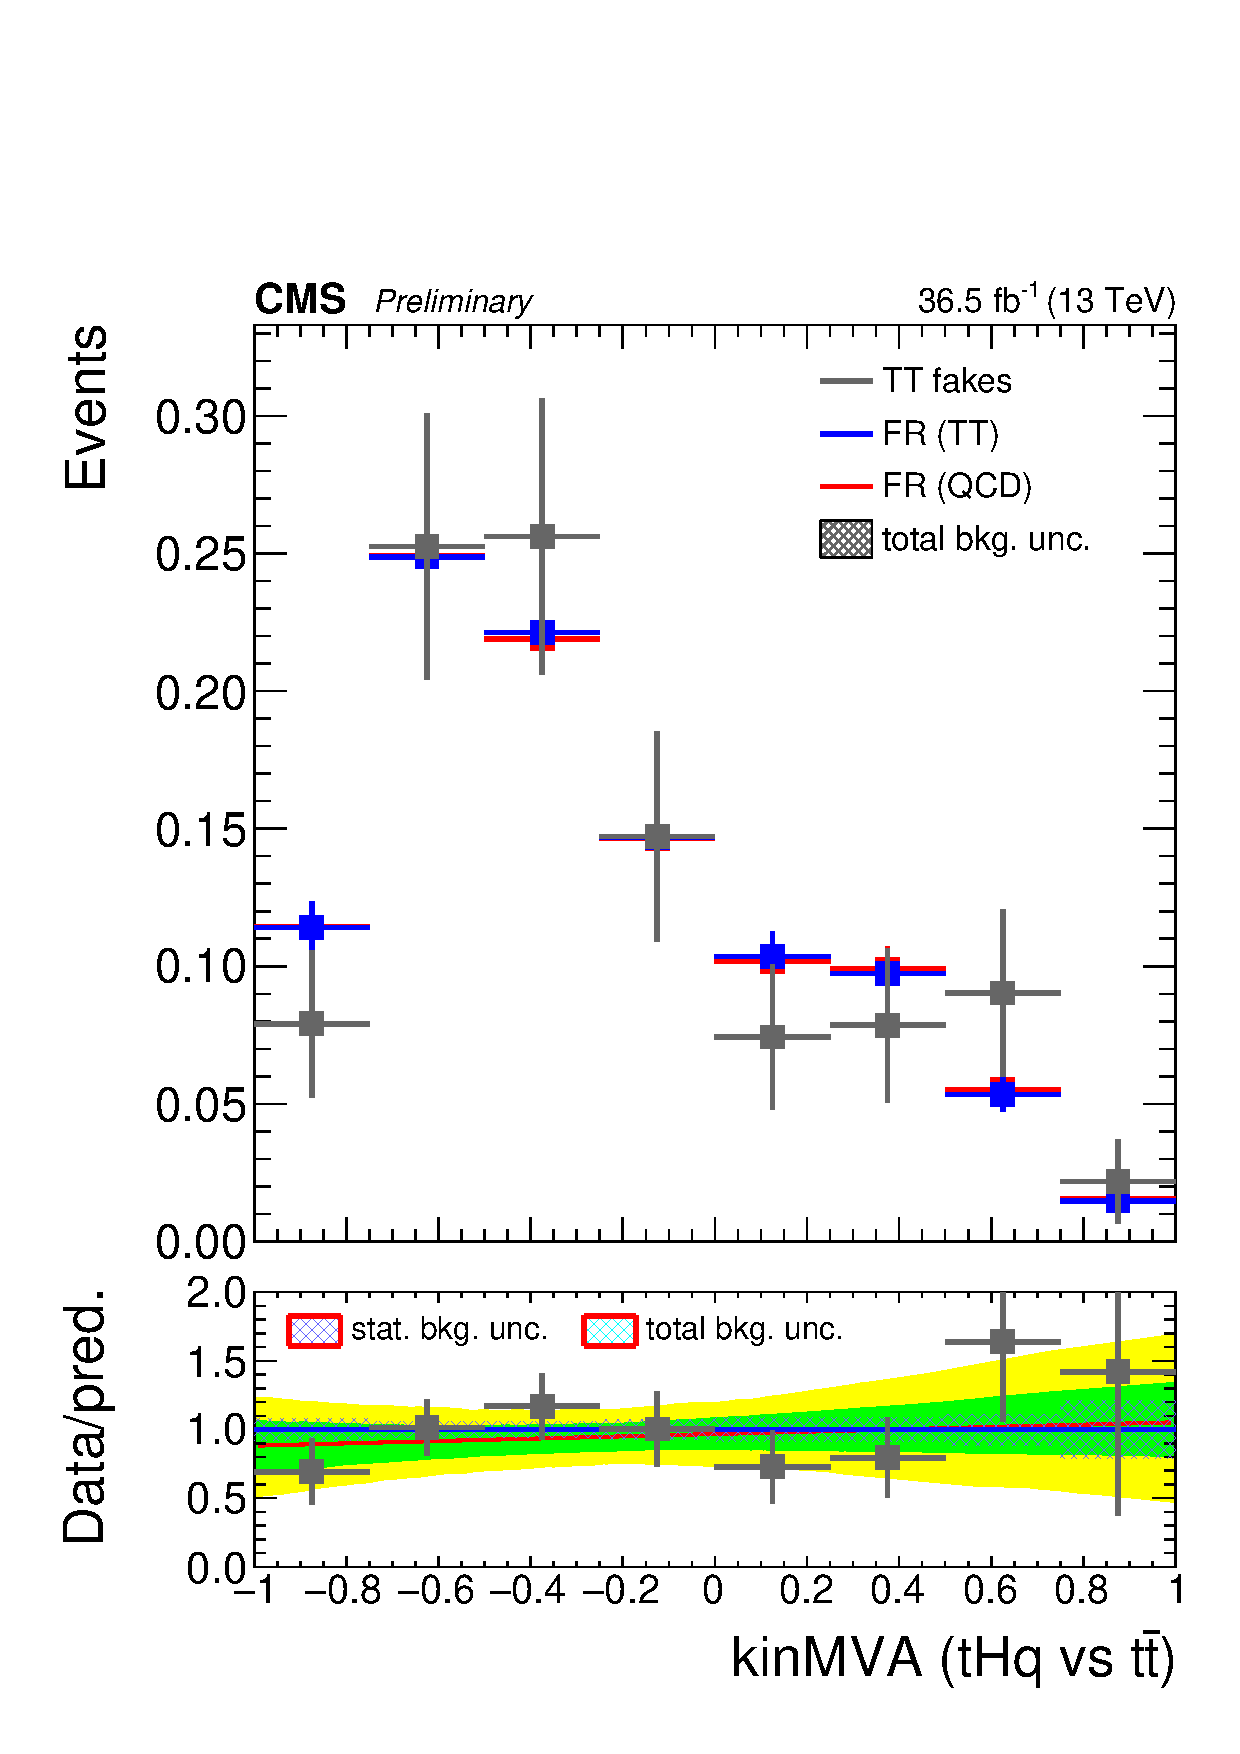
\includegraphics[width=0.245\textwidth]{figures/FR_closures/thqMVA_tt_3l_elfake_shape.pdf} 
 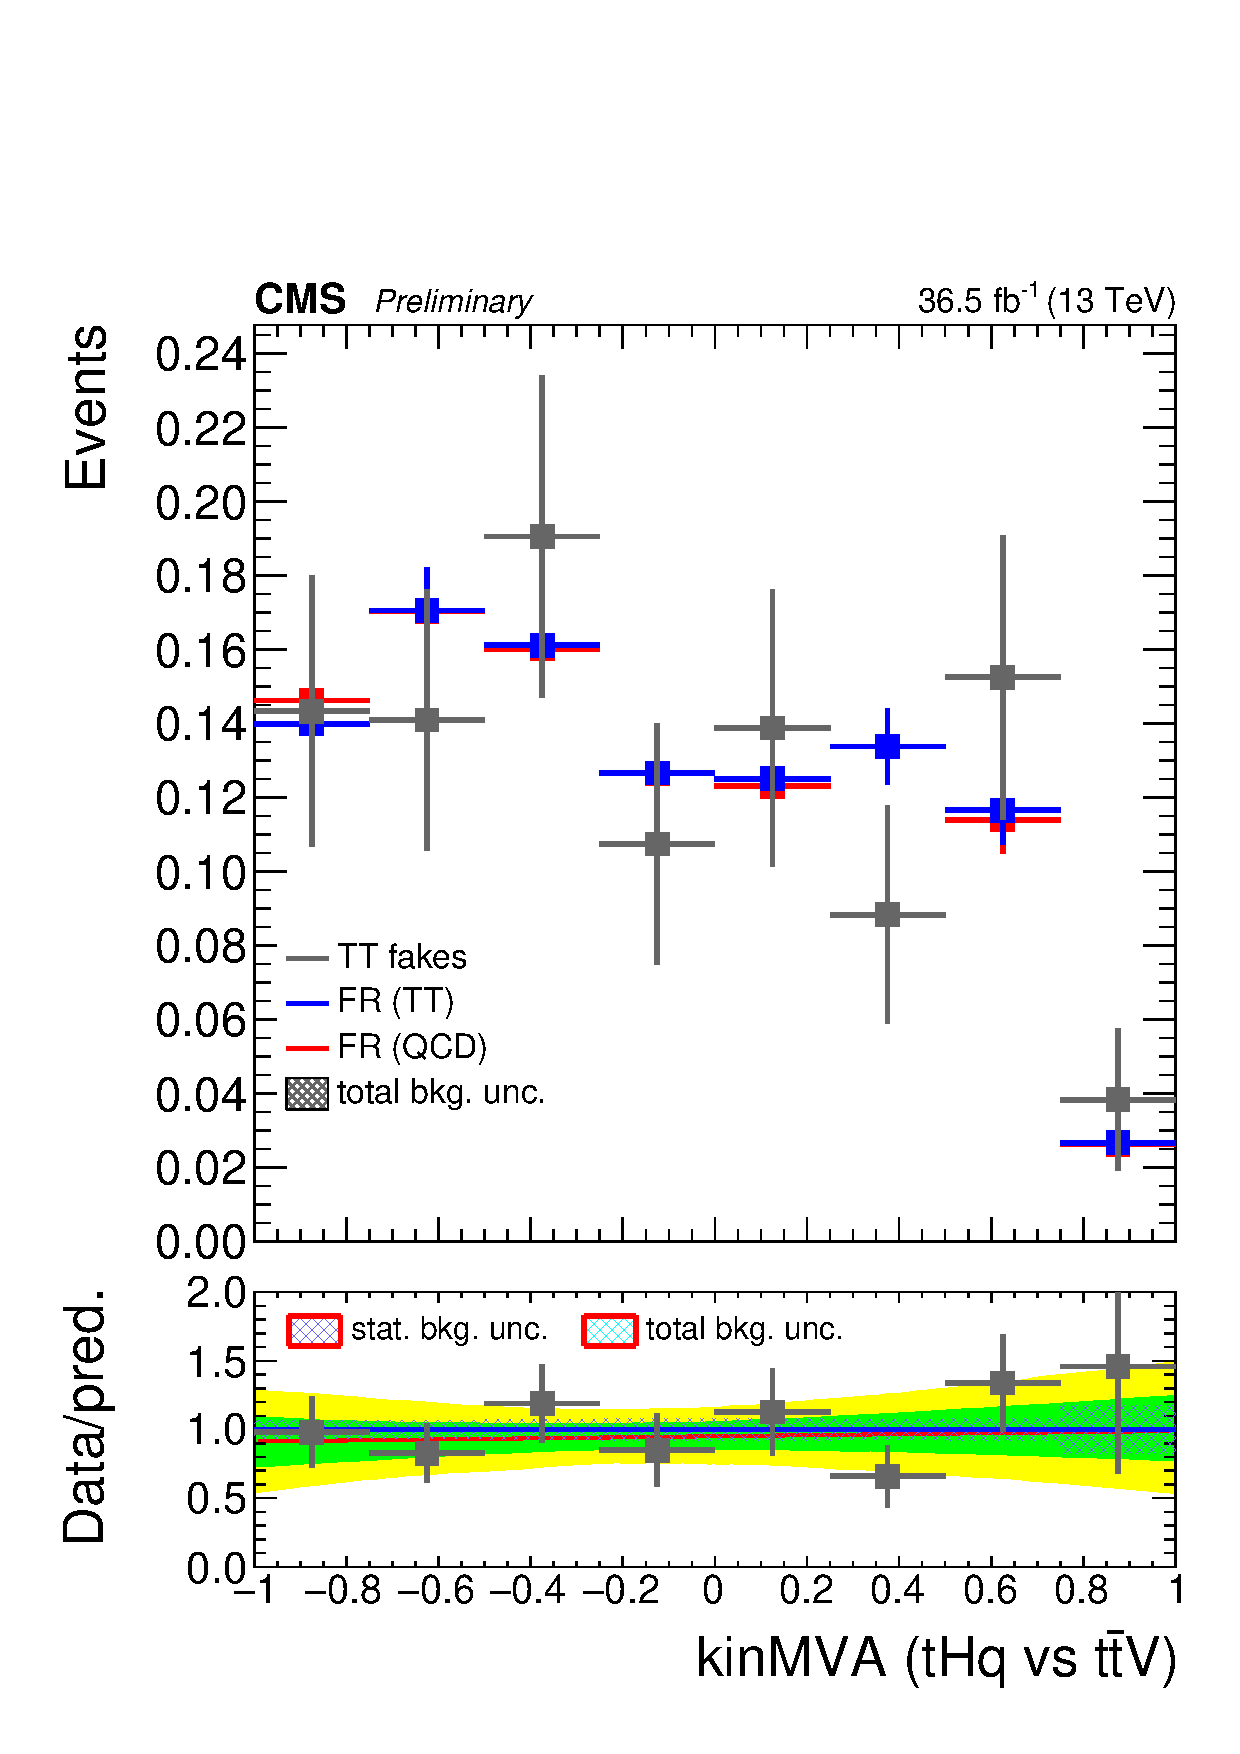
\includegraphics[width=0.245\textwidth]{figures/FR_closures/thqMVA_ttv_3l_elfake_shape.pdf} \\
\caption{BDT outputs comparing \ttbar\ MC to a fake-rate prediction using fake rates measured in QCD MC.\@ Agreement in normalization is estimated from the left two plots, shape disagreement is estimated from the right two (normalized) plots. Three lepton selection with electron fakes.} 
\label{fig:frclosure_3l_elfake}
\end{figure} 

\begin{figure}[htb]
 \centering
 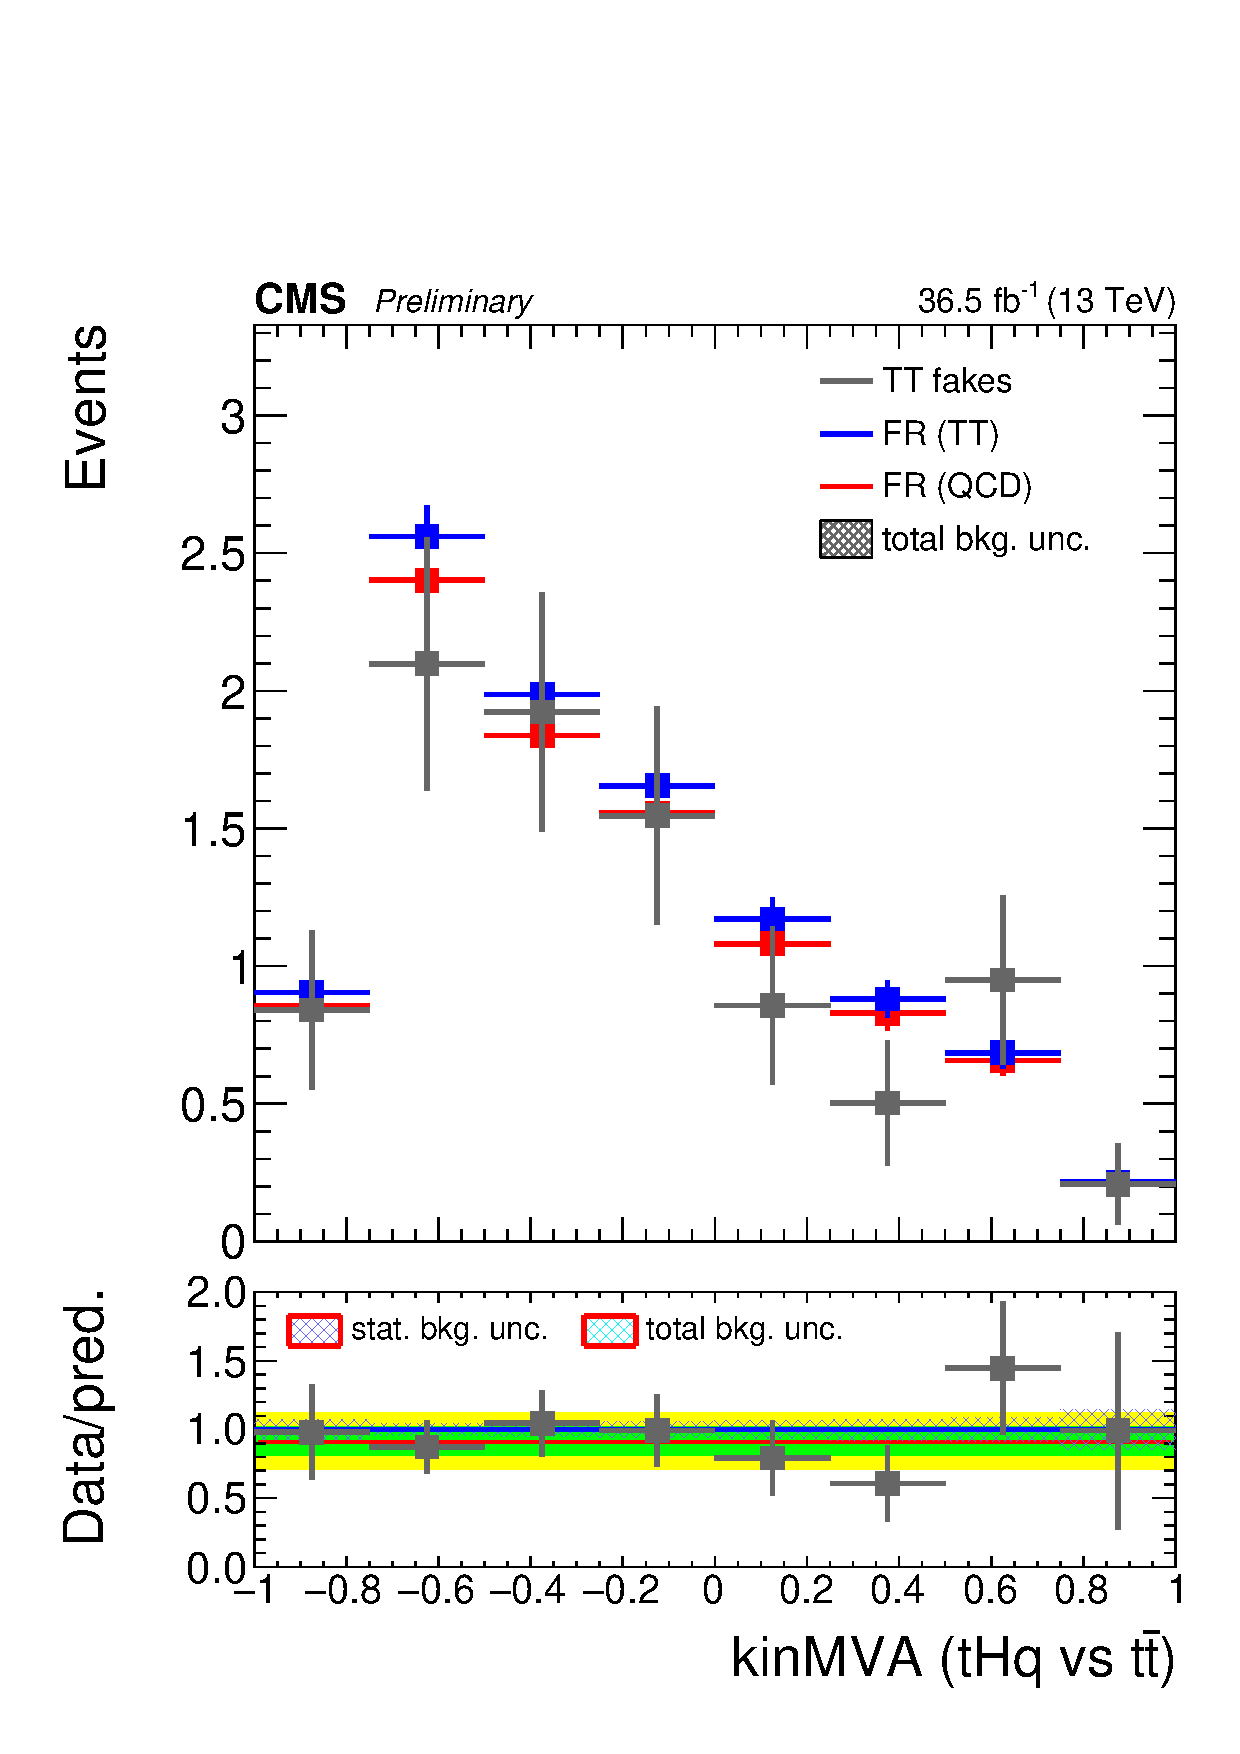
\includegraphics[width=0.245\textwidth]{figures/FR_closures/thqMVA_tt_3l_mufake_norm.pdf} 
 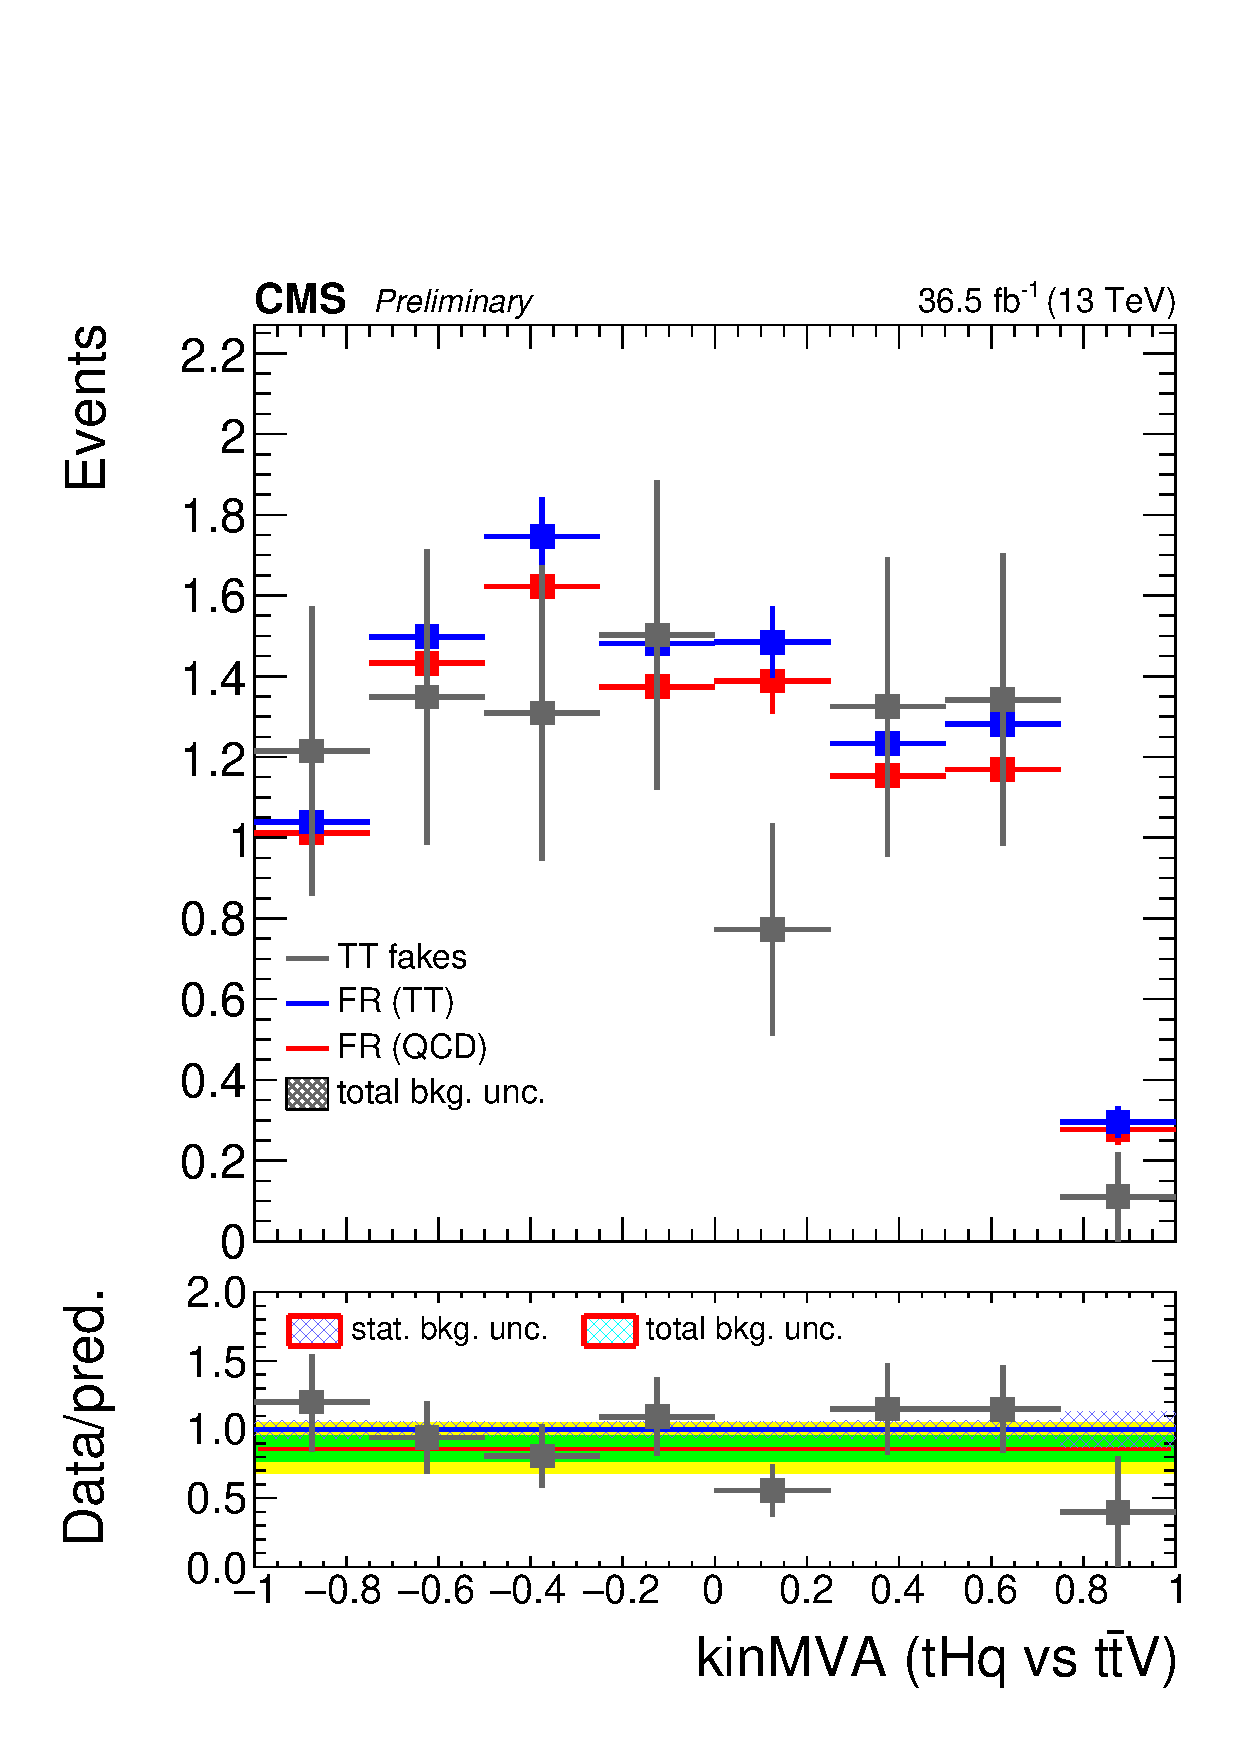
\includegraphics[width=0.245\textwidth]{figures/FR_closures/thqMVA_ttv_3l_mufake_norm.pdf} 
 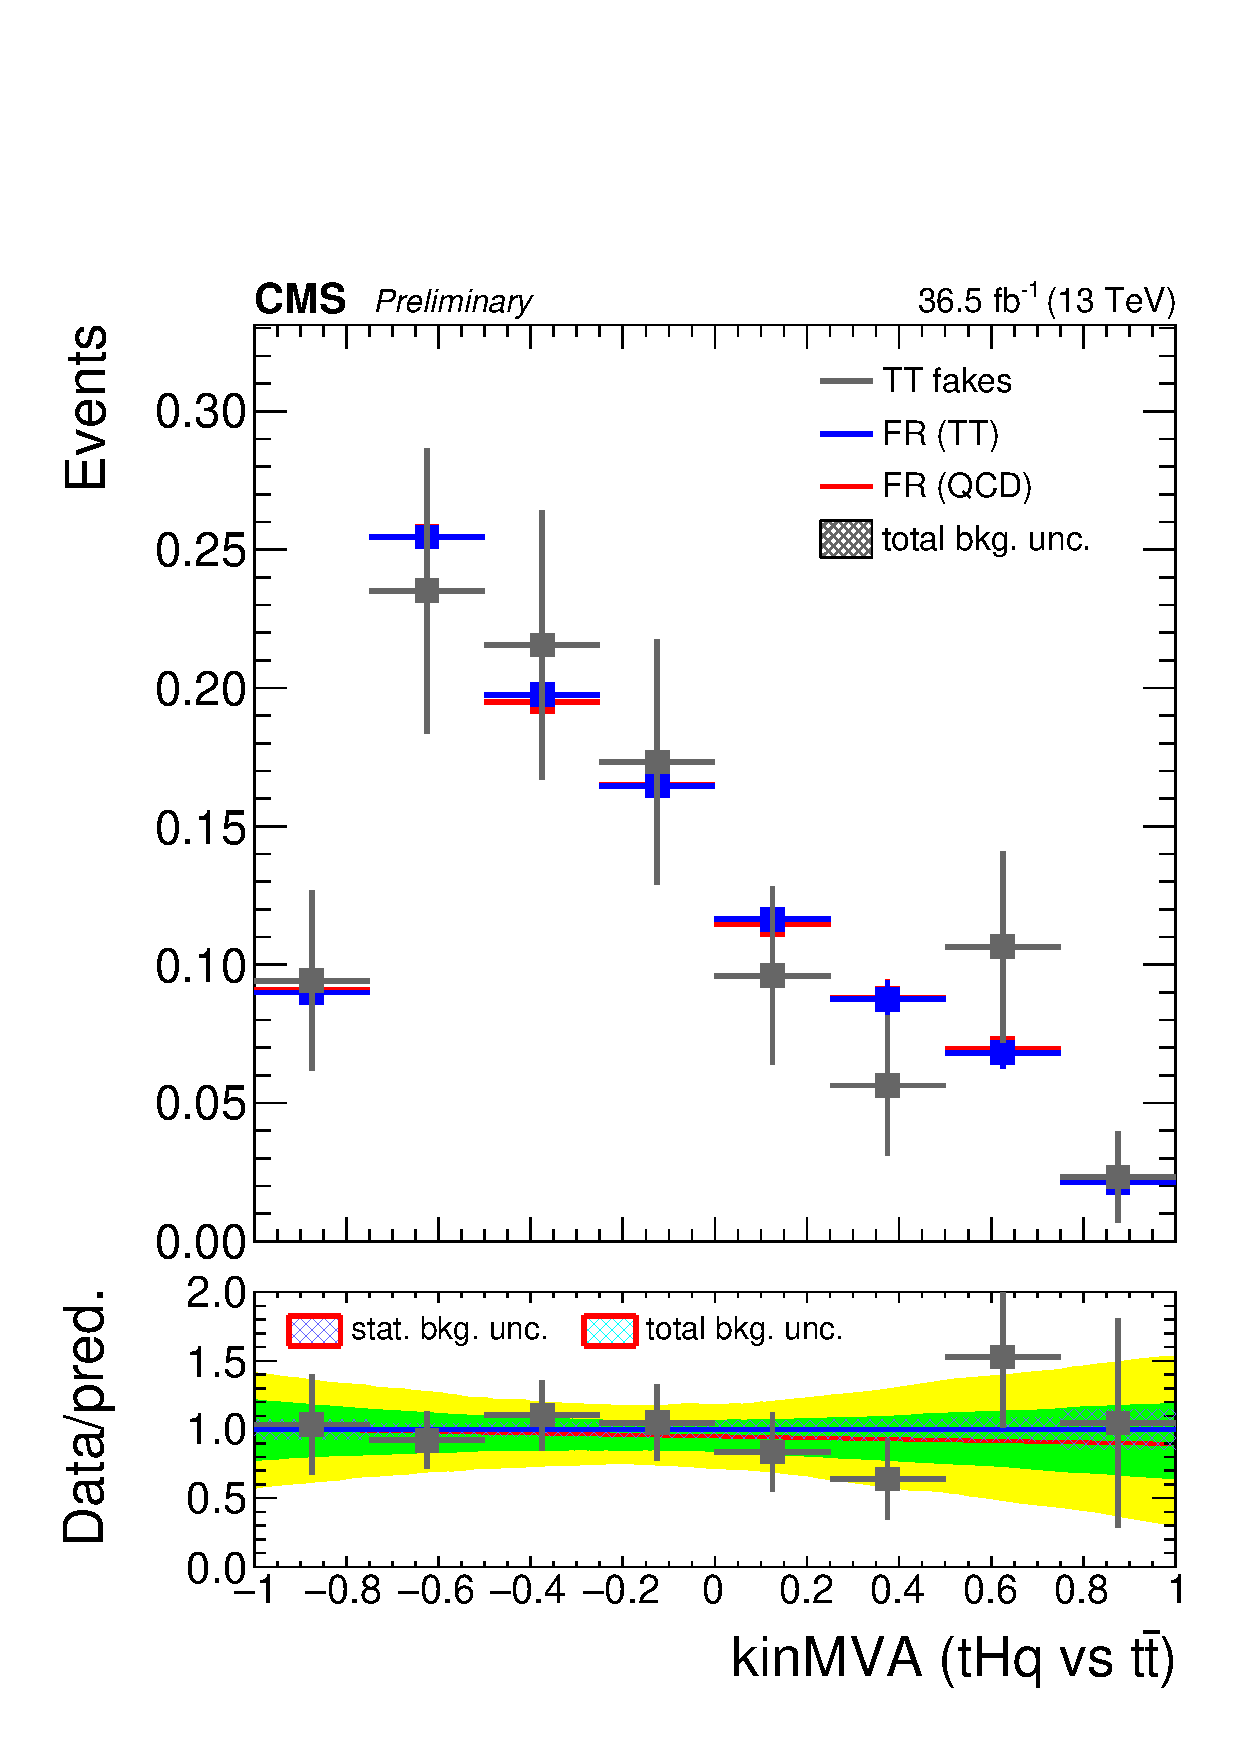
\includegraphics[width=0.245\textwidth]{figures/FR_closures/thqMVA_tt_3l_mufake_shape.pdf} 
 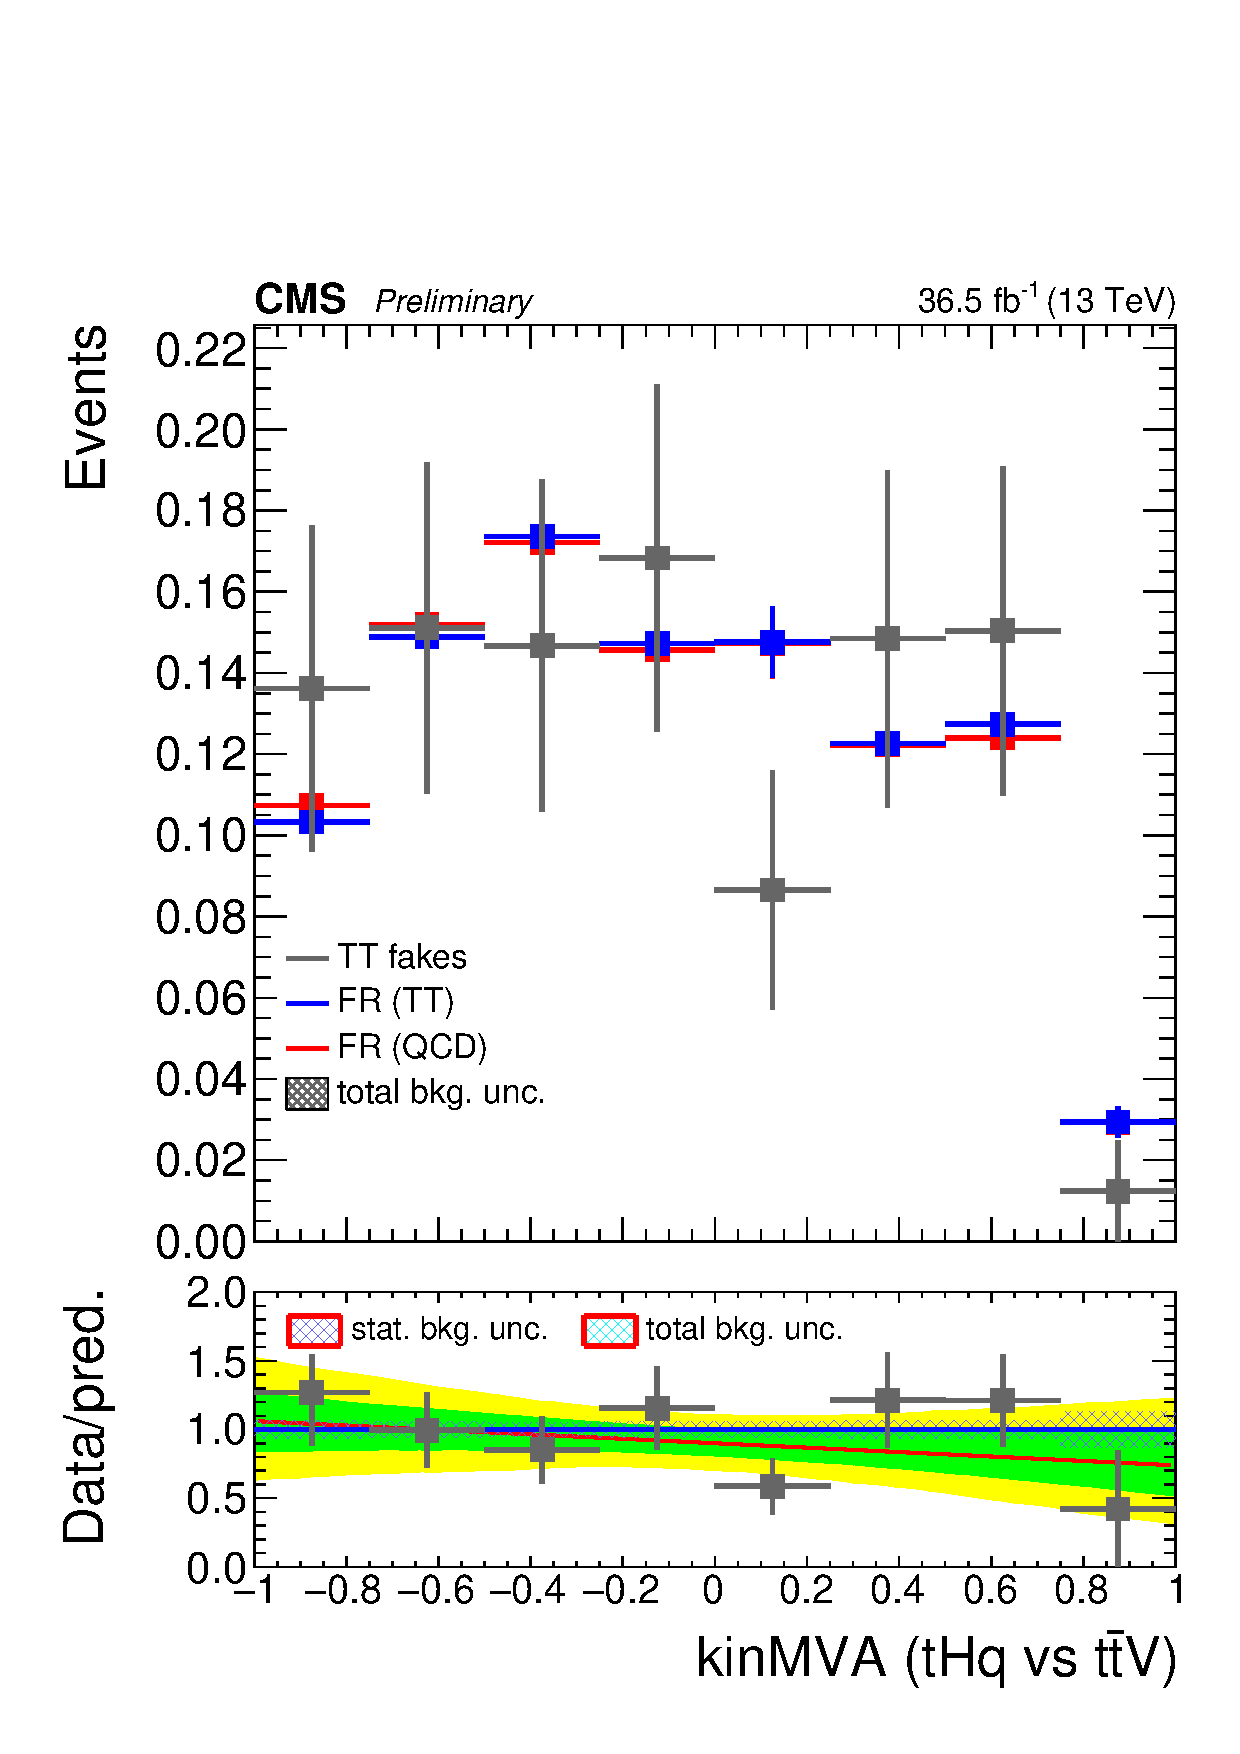
\includegraphics[width=0.245\textwidth]{figures/FR_closures/thqMVA_ttv_3l_mufake_shape.pdf} 
\caption{BDT outputs comparing \ttbar\ MC to a fake-rate prediction using fake rates measured in QCD MC.\@ Agreement in normalization is estimated from the left two plots, shape disagreement is estimated from the right two (normalized) plots. Three lepton selection with muon fakes.} 
\label{fig:frclosure_3l_mufake}
\end{figure}
